%   Filename    : appendix_B.tex

\chapter{Boxplots for All Numeric Features by Feature Family}
\label{app:boxplots_by_family}

This appendix provides boxplots for all numeric features grouped by feature family. These plots complement the selected boxplots shown in Chapter~4 and provide a fuller view of class-specific feature distributions for clean and chimeric reads.

\setlength{\floatsep}{8pt}
\setlength{\textfloatsep}{10pt}
\setlength{\intextsep}{8pt}

\subsection{SA Structure (Supplementary Alignment and Segment Metrics)}
\label{app:boxplots_sa_structure}

\begin{figure}[!htbp]
\centering
\begin{subfigure}[b]{0.32\textwidth}
    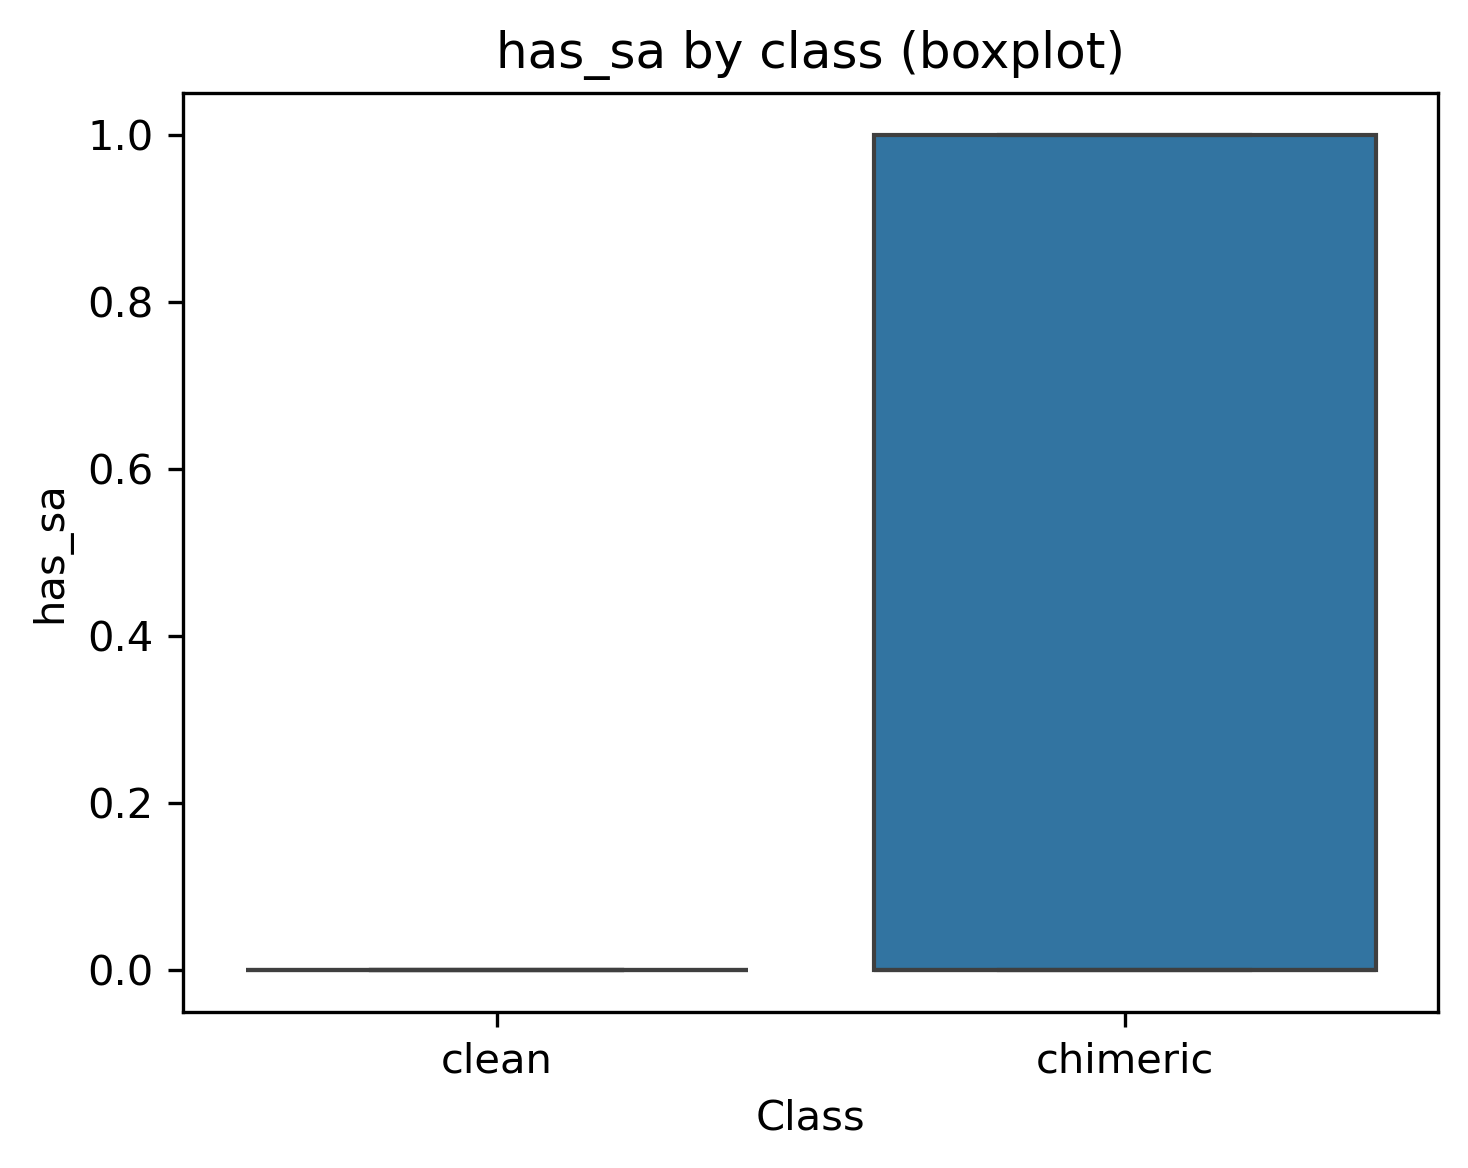
\includegraphics[width=\textwidth]{../notebooks/figures/boxplots/box_has_sa.png}
    \caption{Has SA}
    \label{fig:app_box_has_sa}
\end{subfigure}\hfill
\begin{subfigure}[b]{0.32\textwidth}
    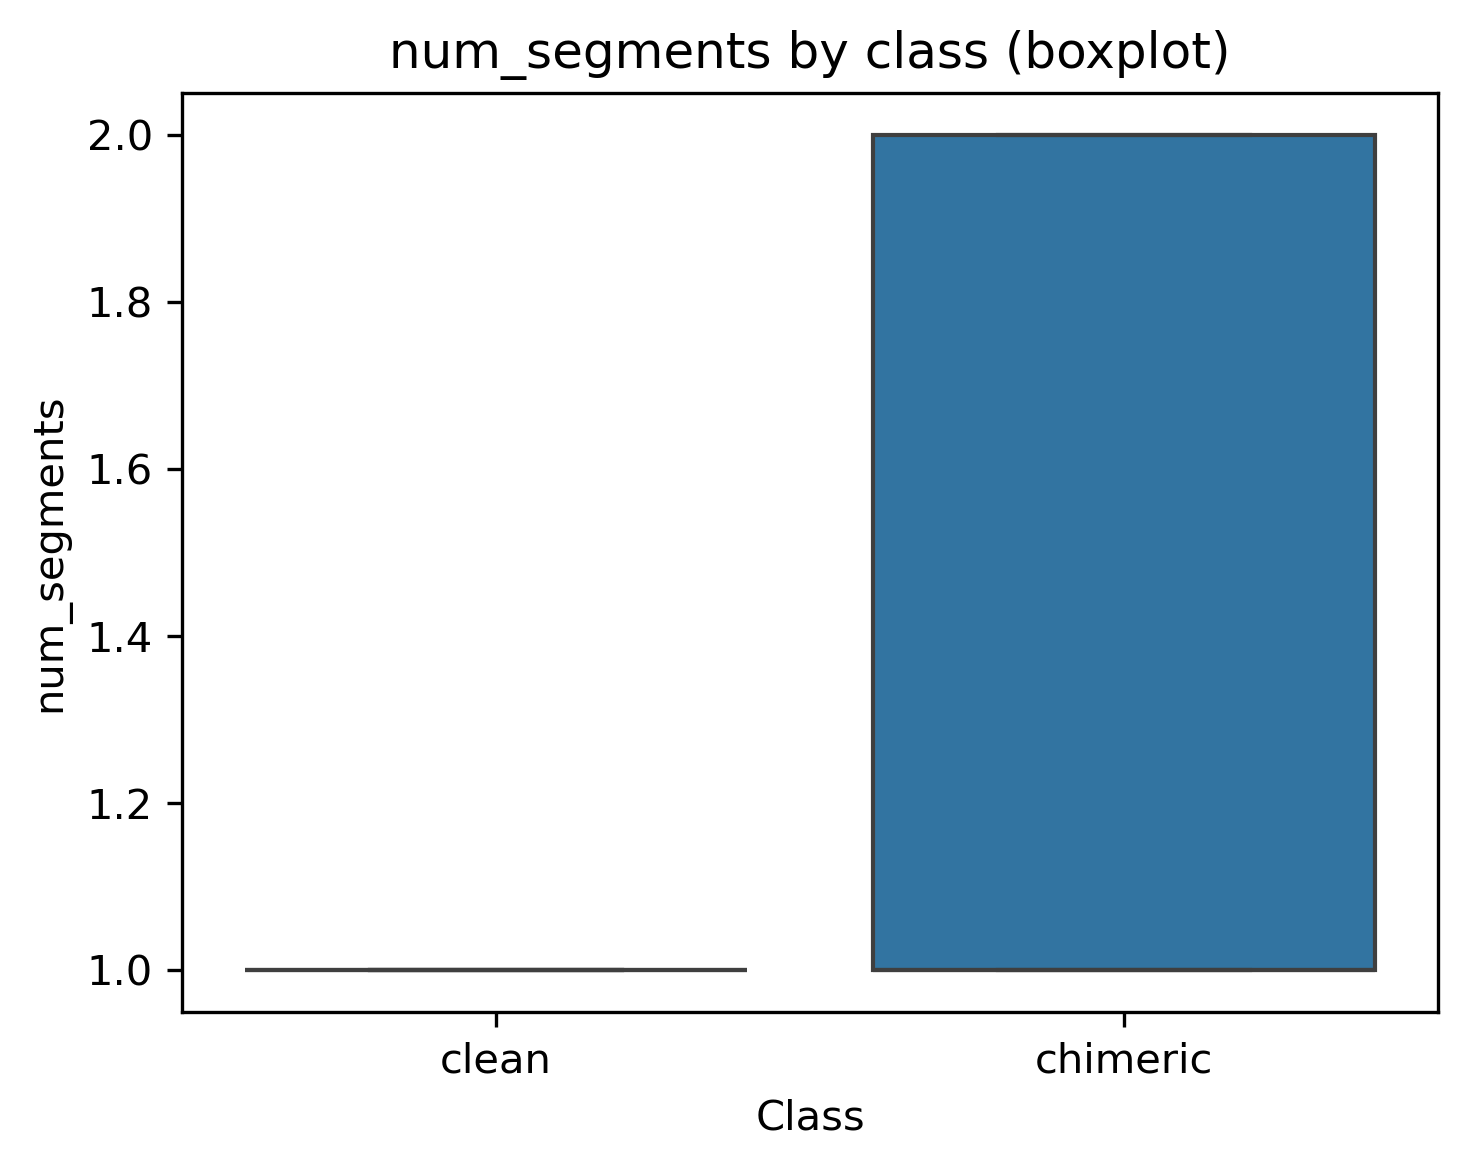
\includegraphics[width=\textwidth]{../notebooks/figures/boxplots/box_num_segments.png}
    \caption{Number of segments}
    \label{fig:app_box_num_segments}
\end{subfigure}\hfill
\begin{subfigure}[b]{0.32\textwidth}
    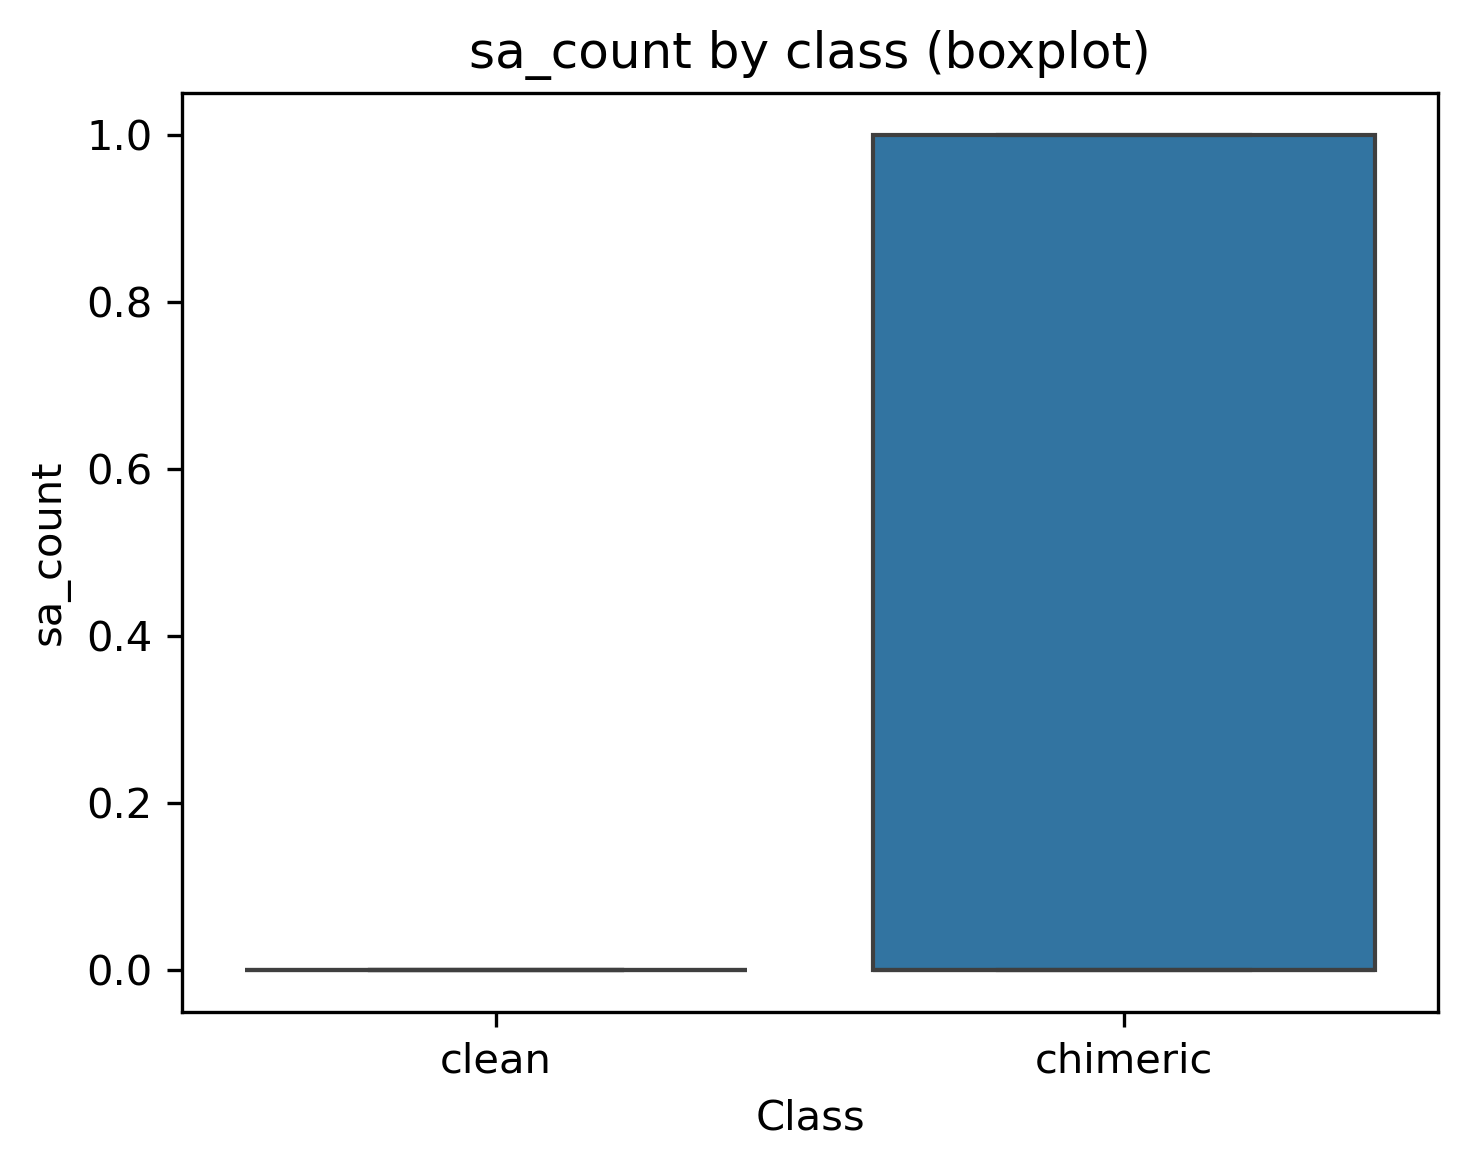
\includegraphics[width=\textwidth]{../notebooks/figures/boxplots/box_sa_count.png}
    \caption{SA count}
    \label{fig:app_box_sa_count}
\end{subfigure}

\caption{Boxplots of SA Structure features by class (1/2).}
\label{fig:app_sa_structure_boxplots_1}
\end{figure}

\begin{figure}[!htbp]
\centering

\begin{subfigure}[b]{0.32\textwidth}
    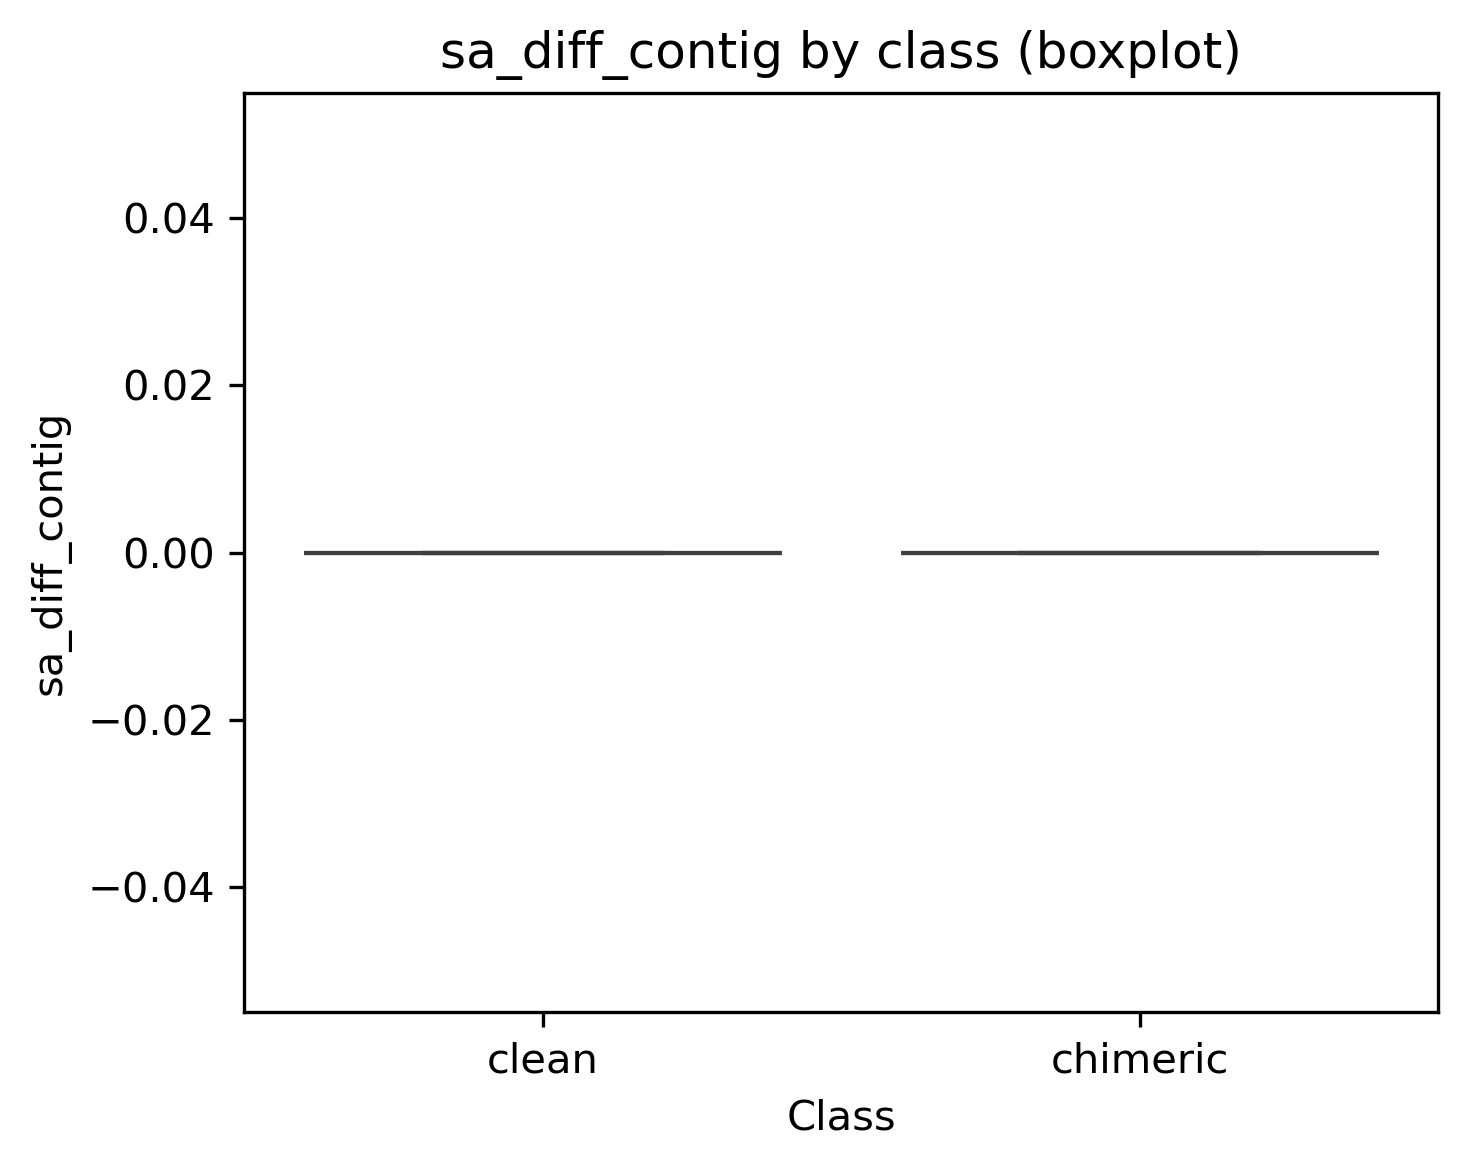
\includegraphics[width=\textwidth]{../notebooks/figures/boxplots/box_sa_diff_contig.png}
    \caption{SA different contig}
    \label{fig:app_box_sa_diff_contig}
\end{subfigure}\hfill
\begin{subfigure}[b]{0.32\textwidth}
    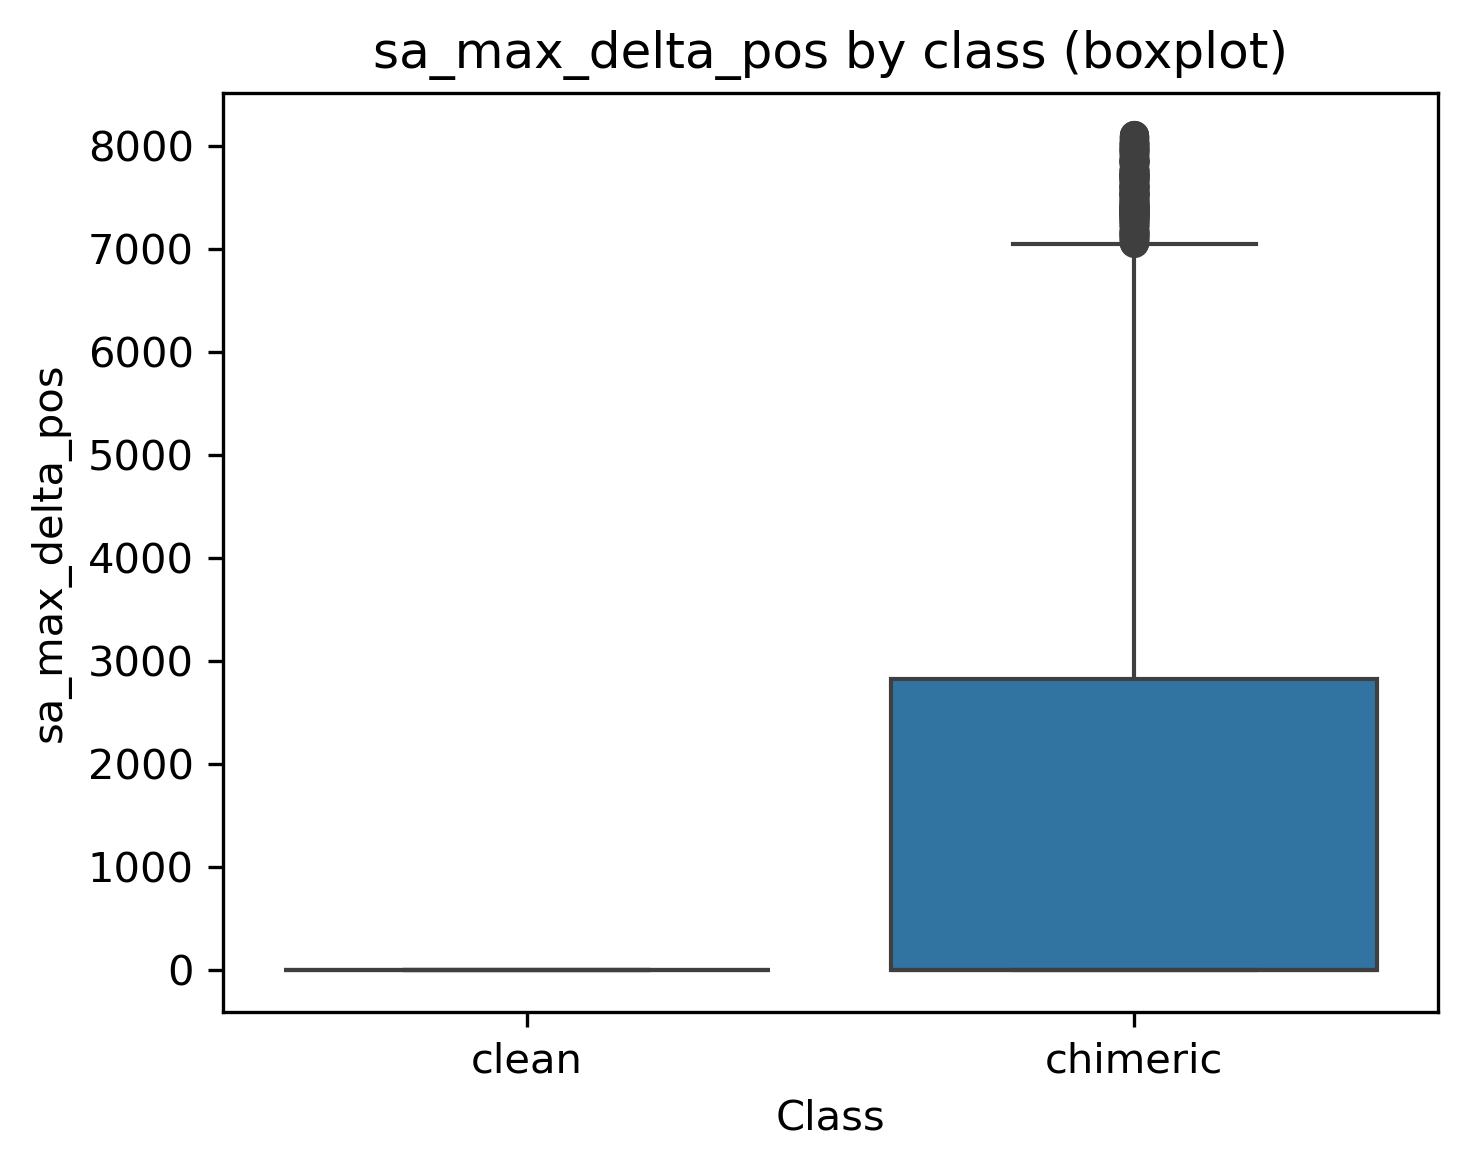
\includegraphics[width=\textwidth]{../notebooks/figures/boxplots/box_sa_max_delta_pos.png}
    \caption{SA max $\Delta$ position}
    \label{fig:app_box_sa_max_delta_pos}
\end{subfigure}\hfill
\begin{subfigure}[b]{0.32\textwidth}
    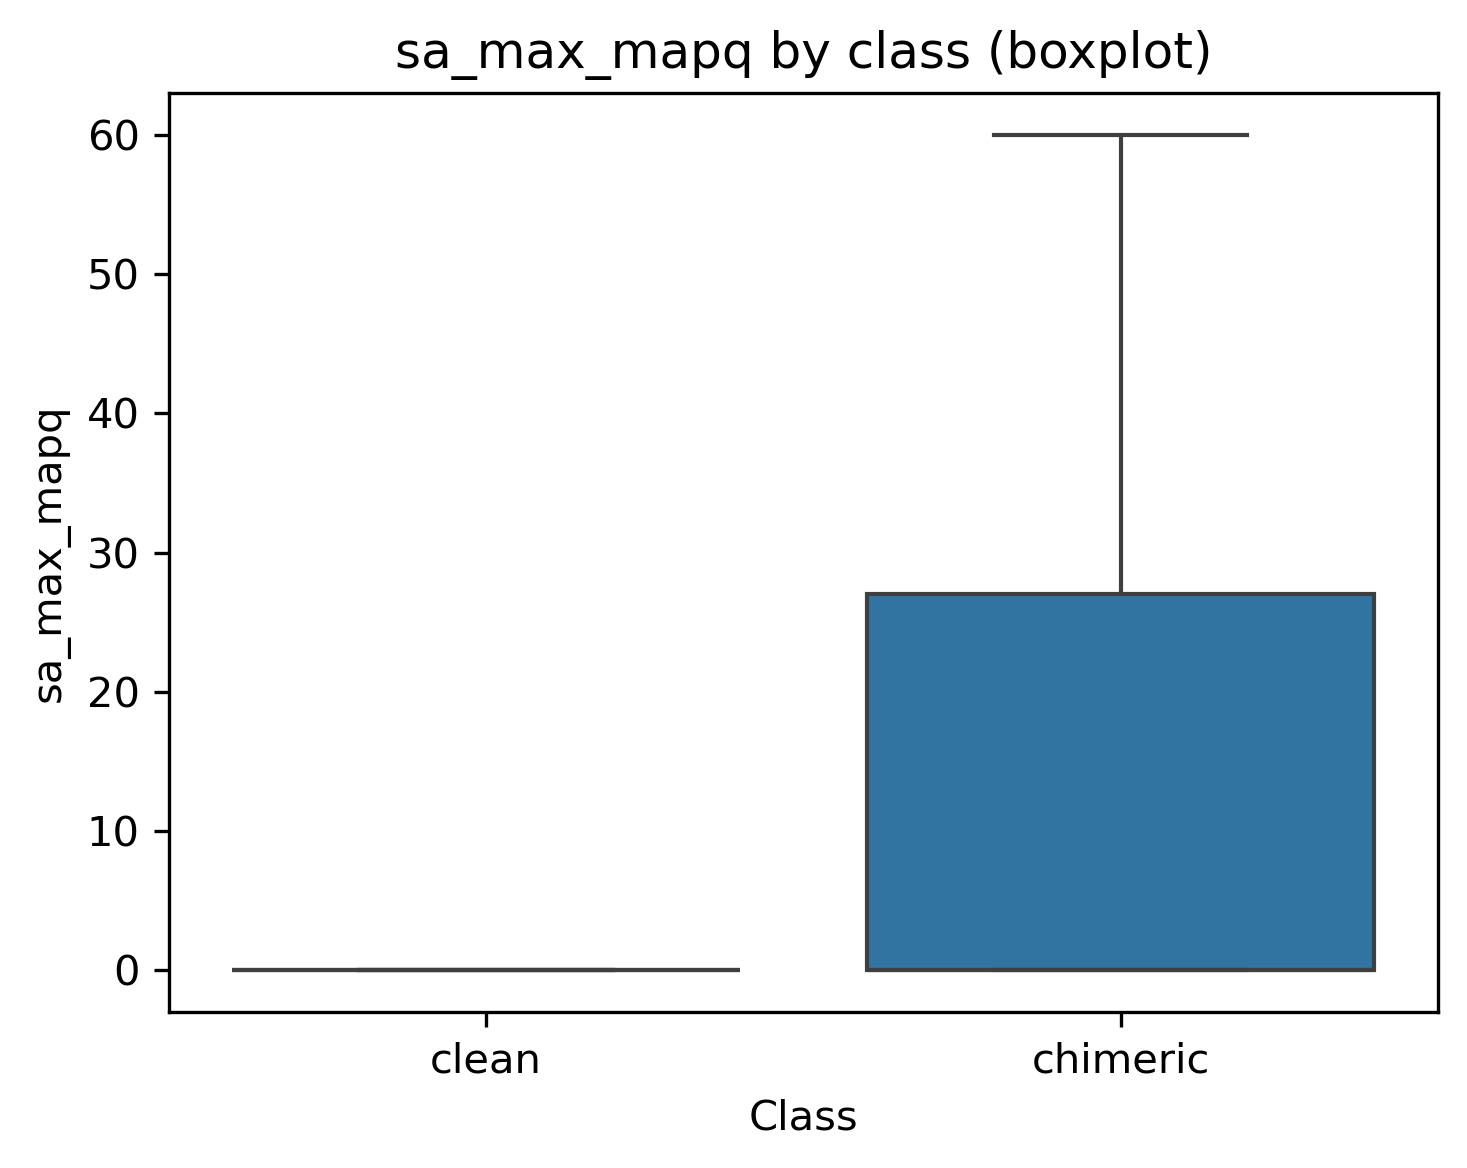
\includegraphics[width=\textwidth]{../notebooks/figures/boxplots/box_sa_max_mapq.png}
    \caption{SA max MAPQ}
    \label{fig:app_box_sa_max_mapq}
\end{subfigure}

\vspace{0.4em}

\begin{subfigure}[b]{0.32\textwidth}
    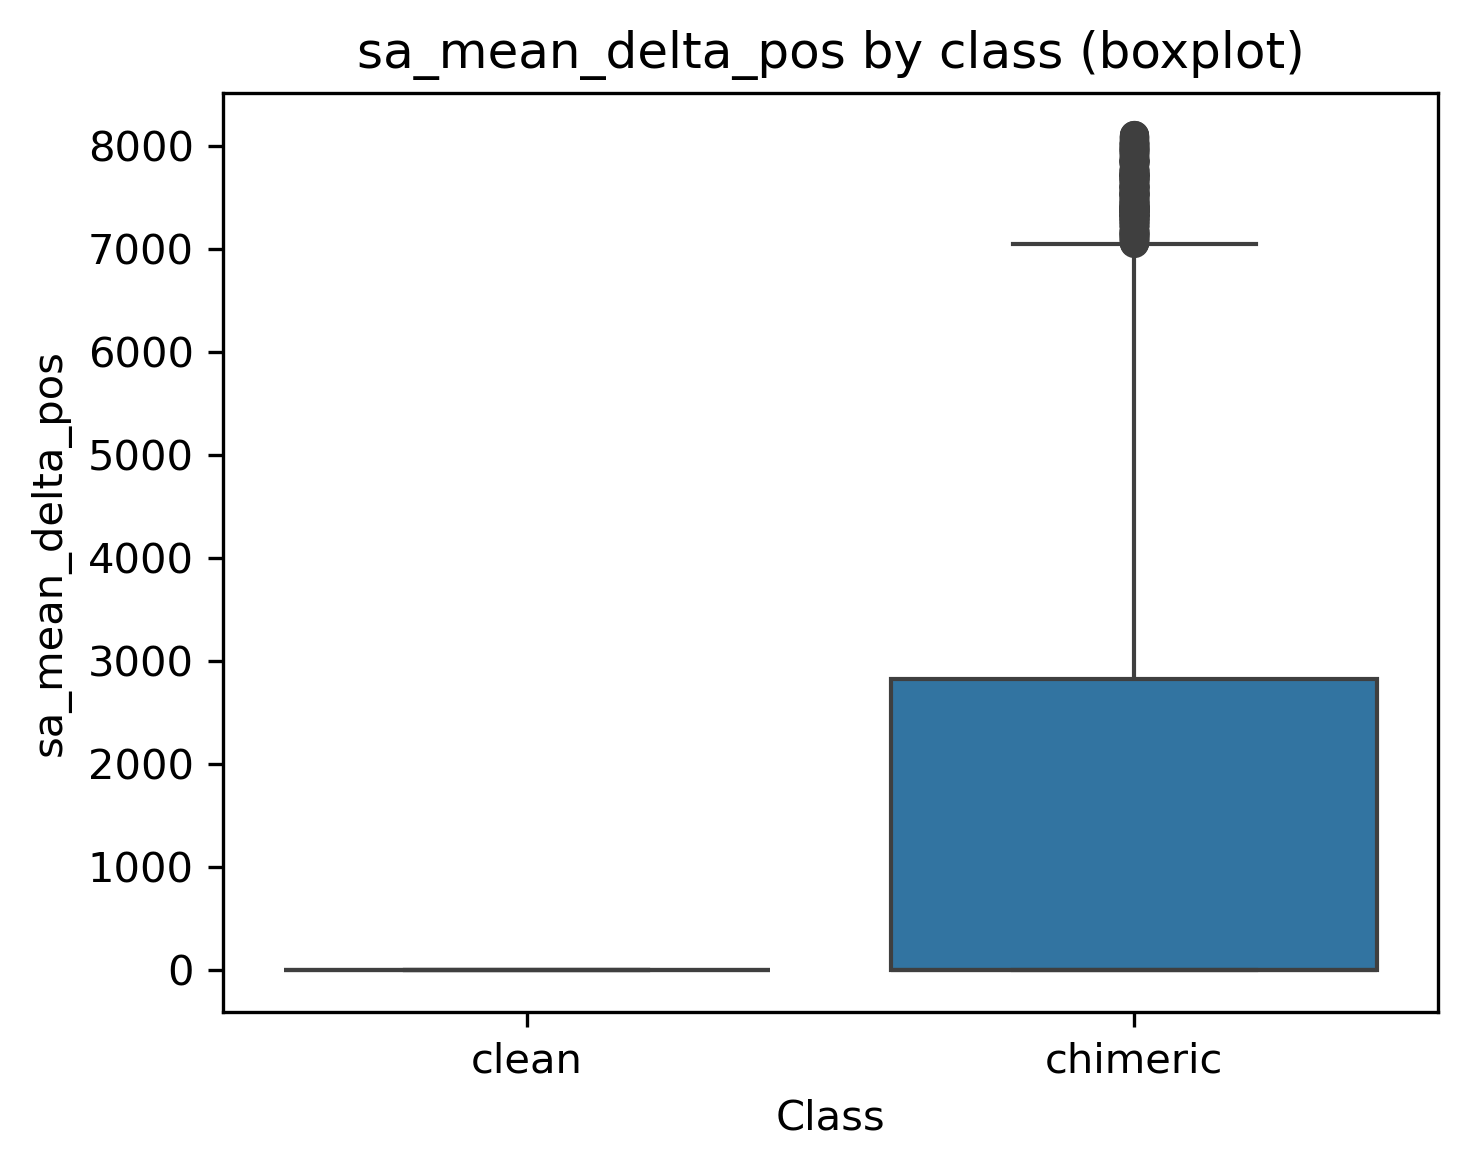
\includegraphics[width=\textwidth]{../notebooks/figures/boxplots/box_sa_mean_delta_pos.png}
    \caption{SA mean $\Delta$ position}
    \label{fig:app_box_sa_mean_delta_pos}
\end{subfigure}\hfill
\begin{subfigure}[b]{0.32\textwidth}
    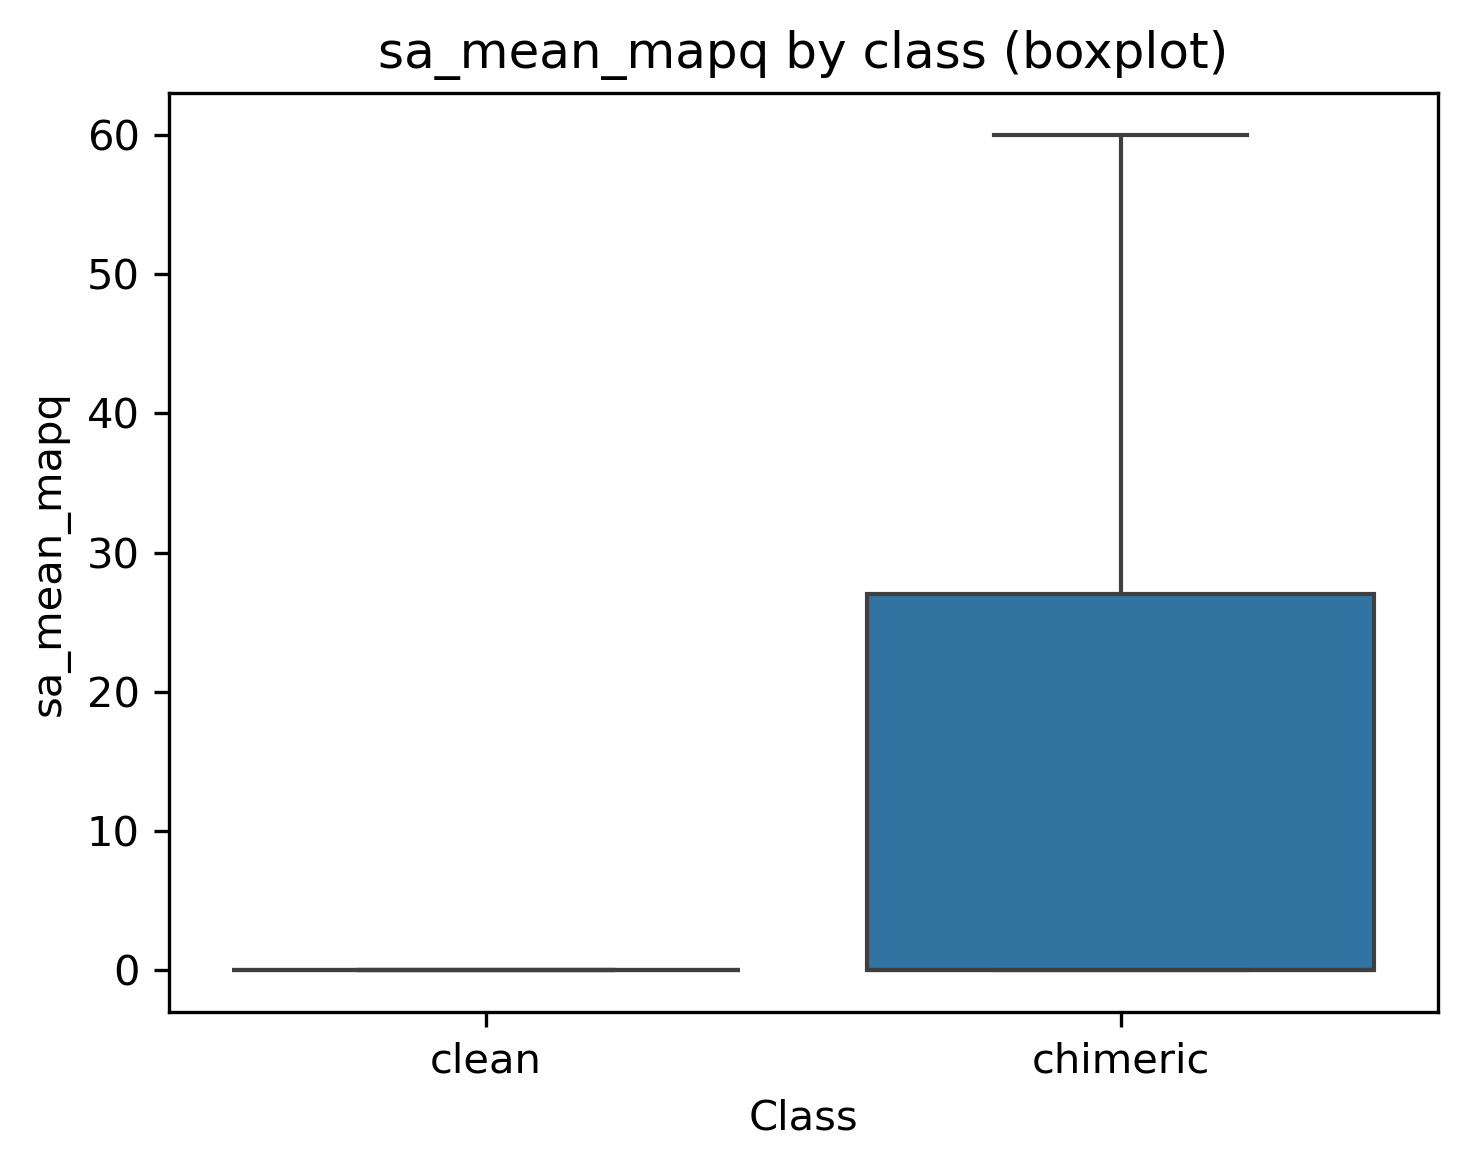
\includegraphics[width=\textwidth]{../notebooks/figures/boxplots/box_sa_mean_mapq.png}
    \caption{SA mean MAPQ}
    \label{fig:app_box_sa_mean_mapq}
\end{subfigure}\hfill
\begin{subfigure}[b]{0.32\textwidth}
    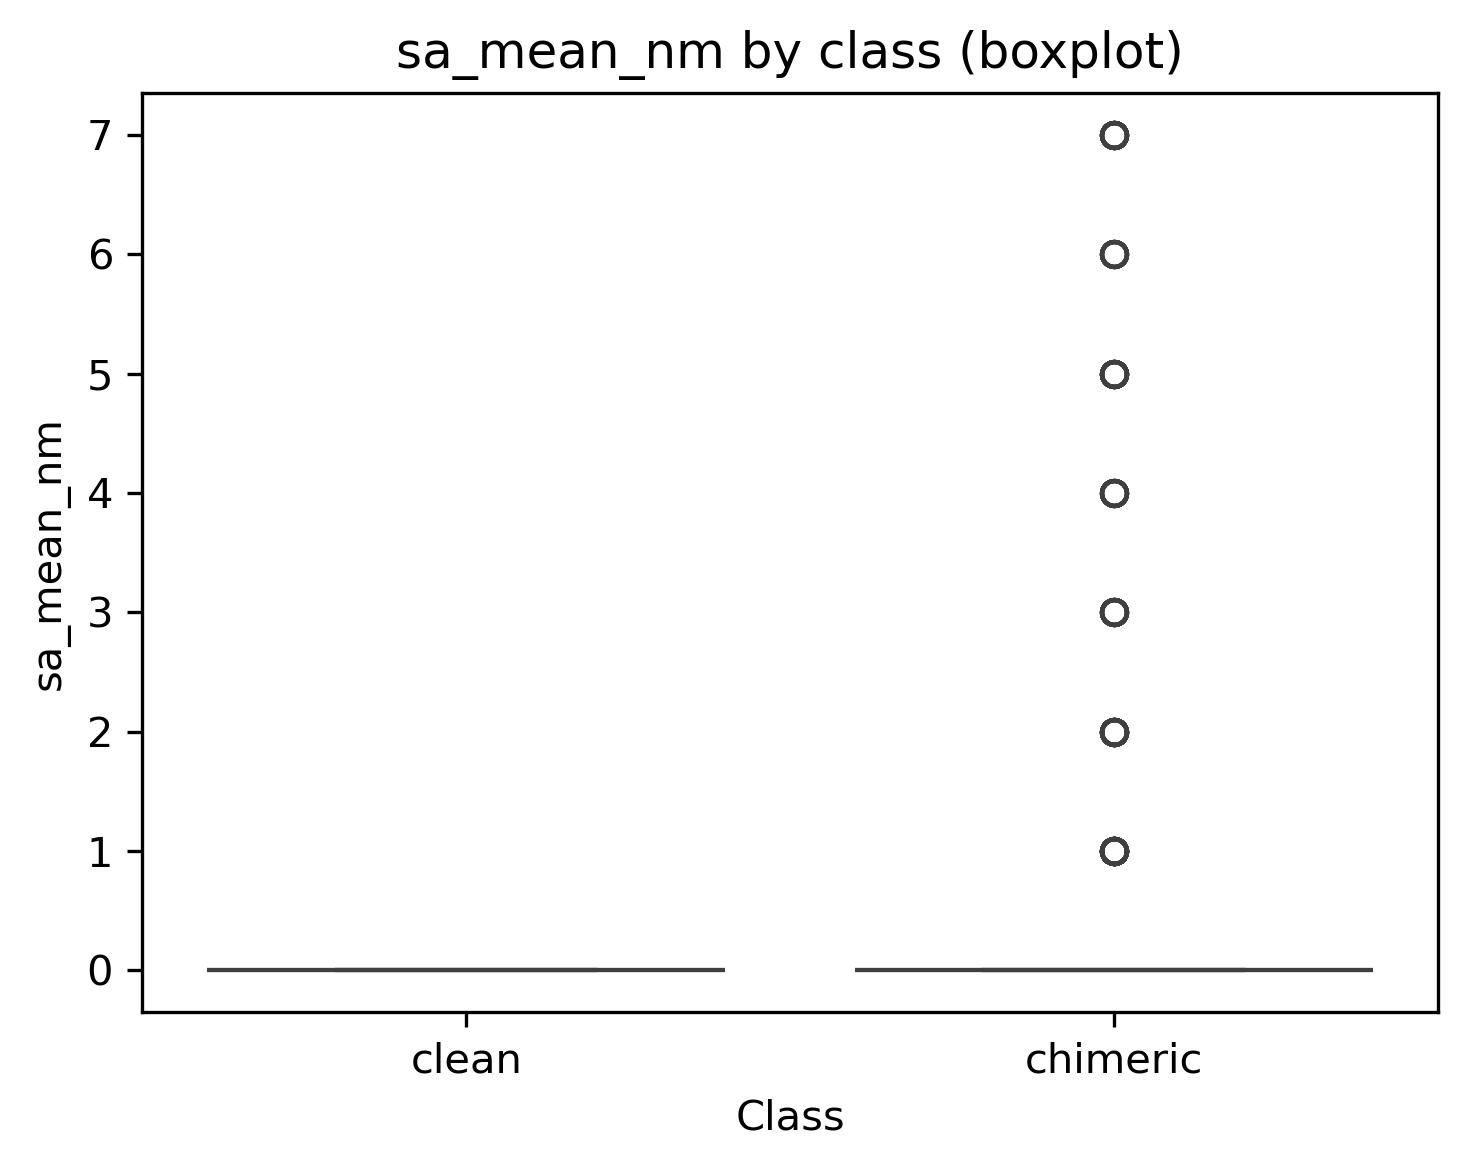
\includegraphics[width=\textwidth]{../notebooks/figures/boxplots/box_sa_mean_nm.png}
    \caption{SA mean NM}
    \label{fig:app_box_sa_mean_nm}
\end{subfigure}

\vspace{0.4em}

\begin{subfigure}[b]{0.32\textwidth}
    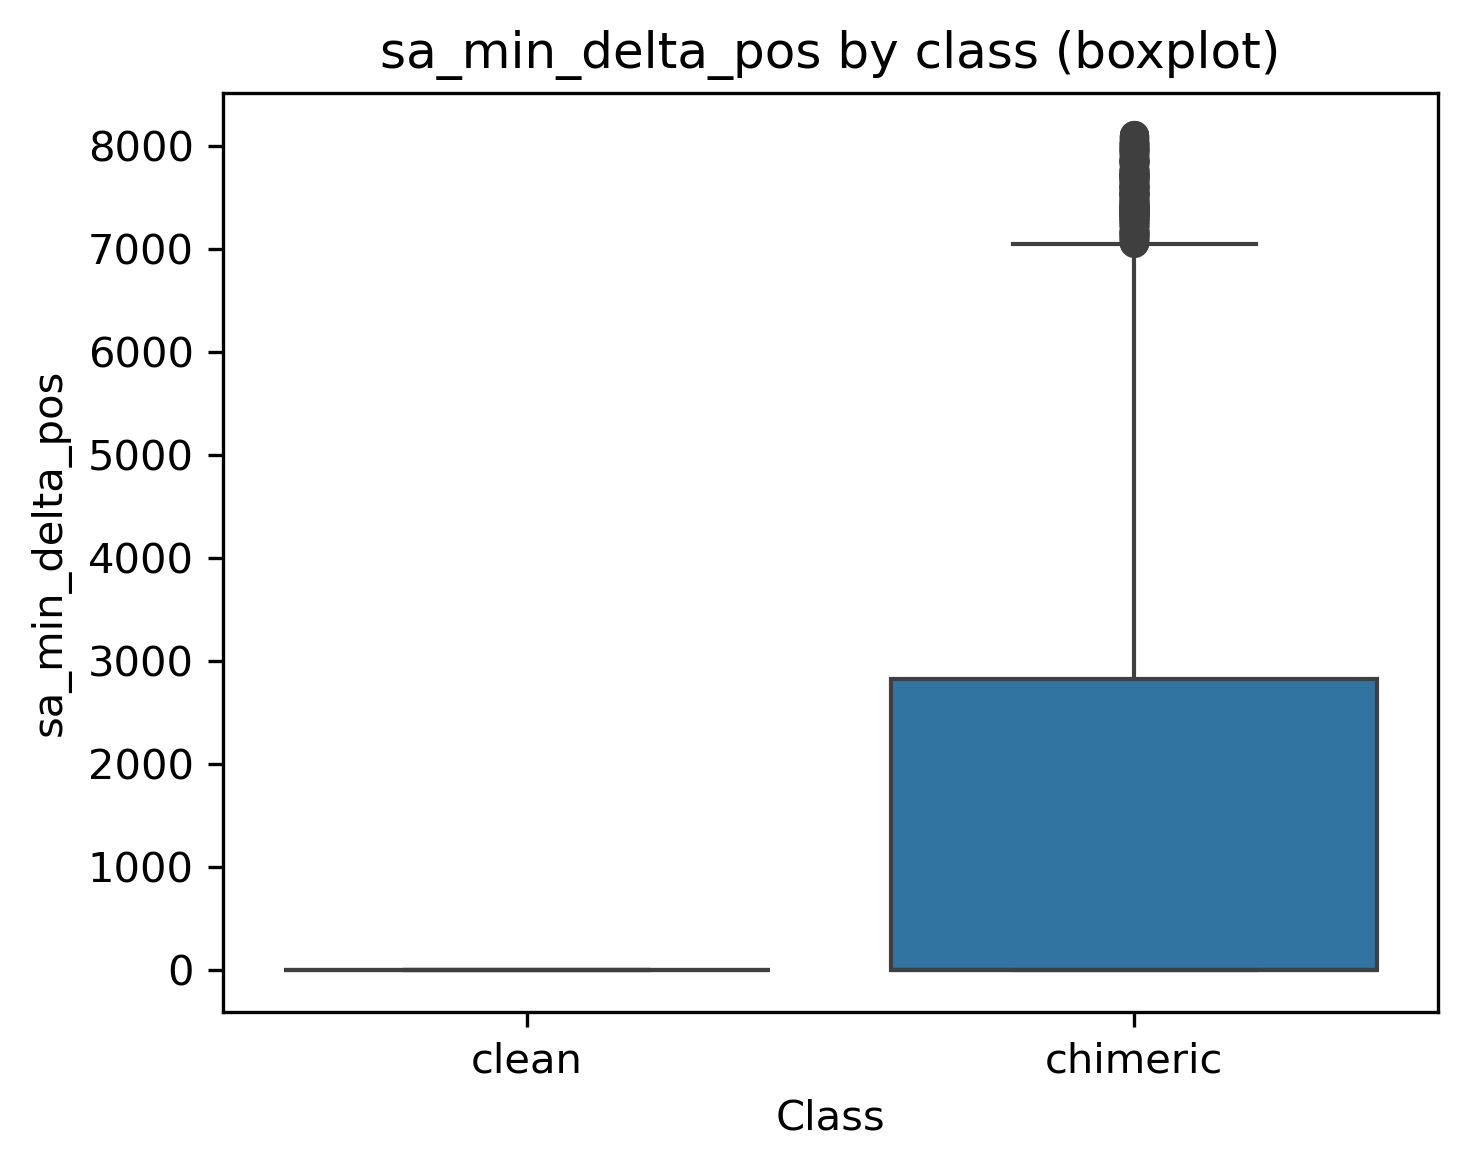
\includegraphics[width=\textwidth]{../notebooks/figures/boxplots/box_sa_min_delta_pos.png}
    \caption{SA min $\Delta$ position}
    \label{fig:app_box_sa_min_delta_pos}
\end{subfigure}\hfill
\begin{subfigure}[b]{0.32\textwidth}
    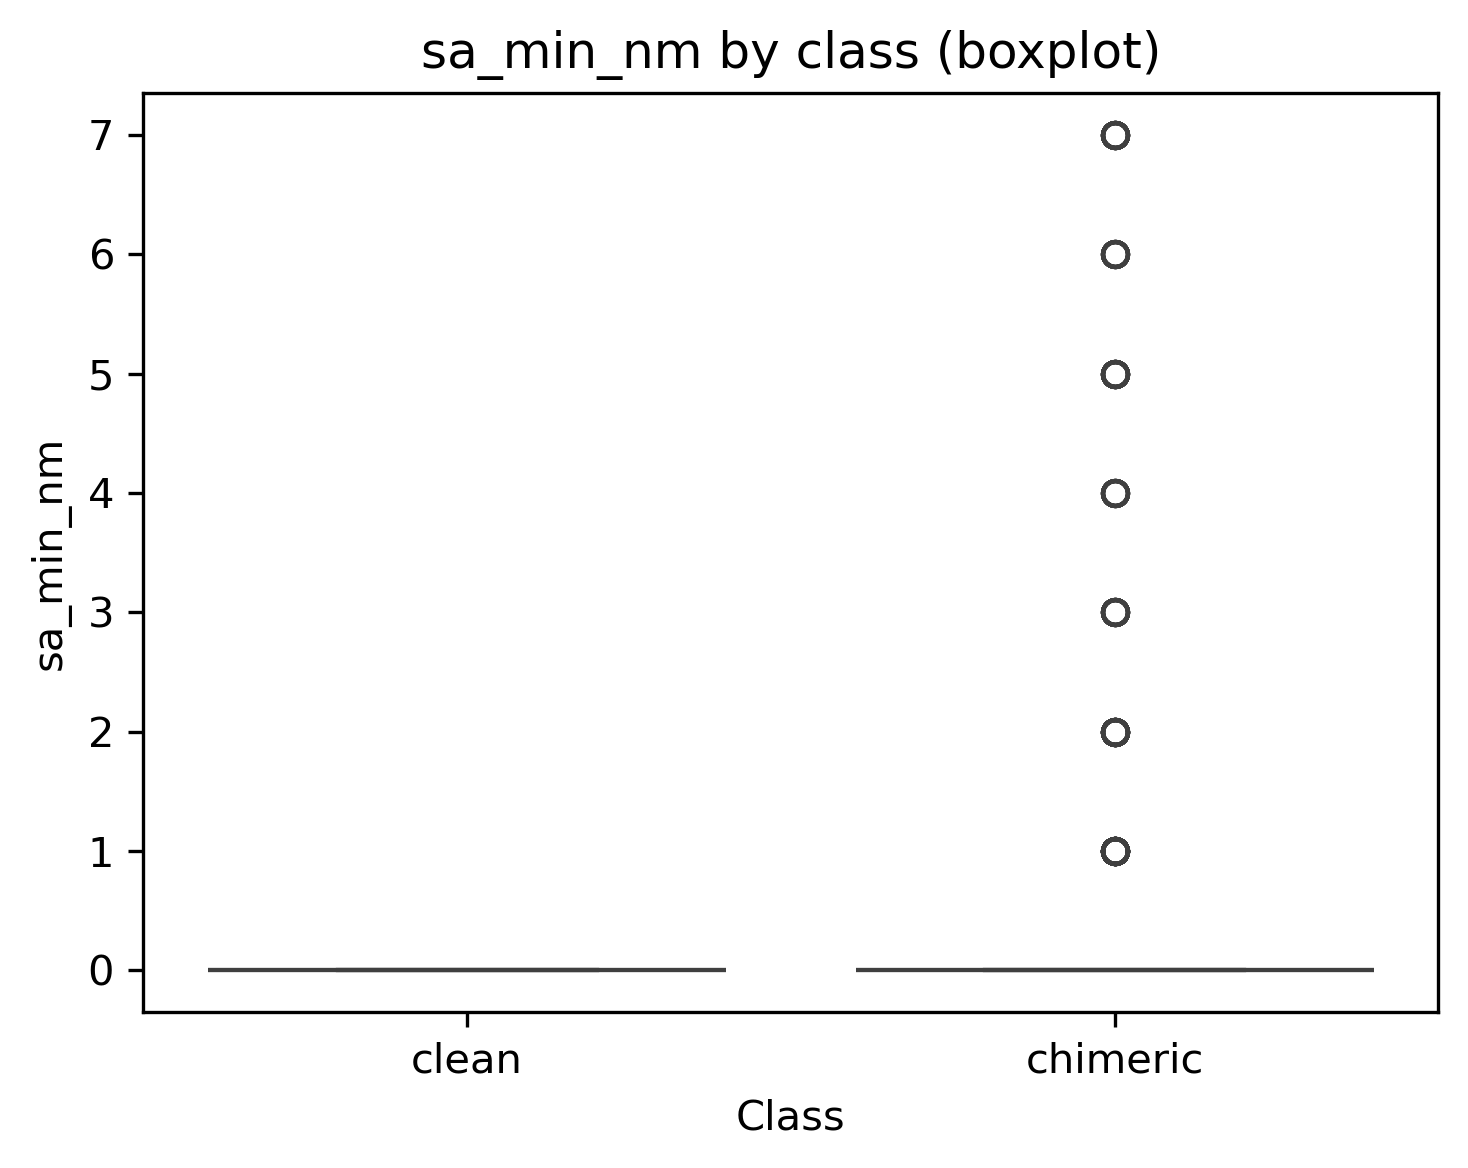
\includegraphics[width=\textwidth]{../notebooks/figures/boxplots/box_sa_min_nm.png}
    \caption{SA min NM}
    \label{fig:app_box_sa_min_nm}
\end{subfigure}\hfill
\begin{subfigure}[b]{0.32\textwidth}
    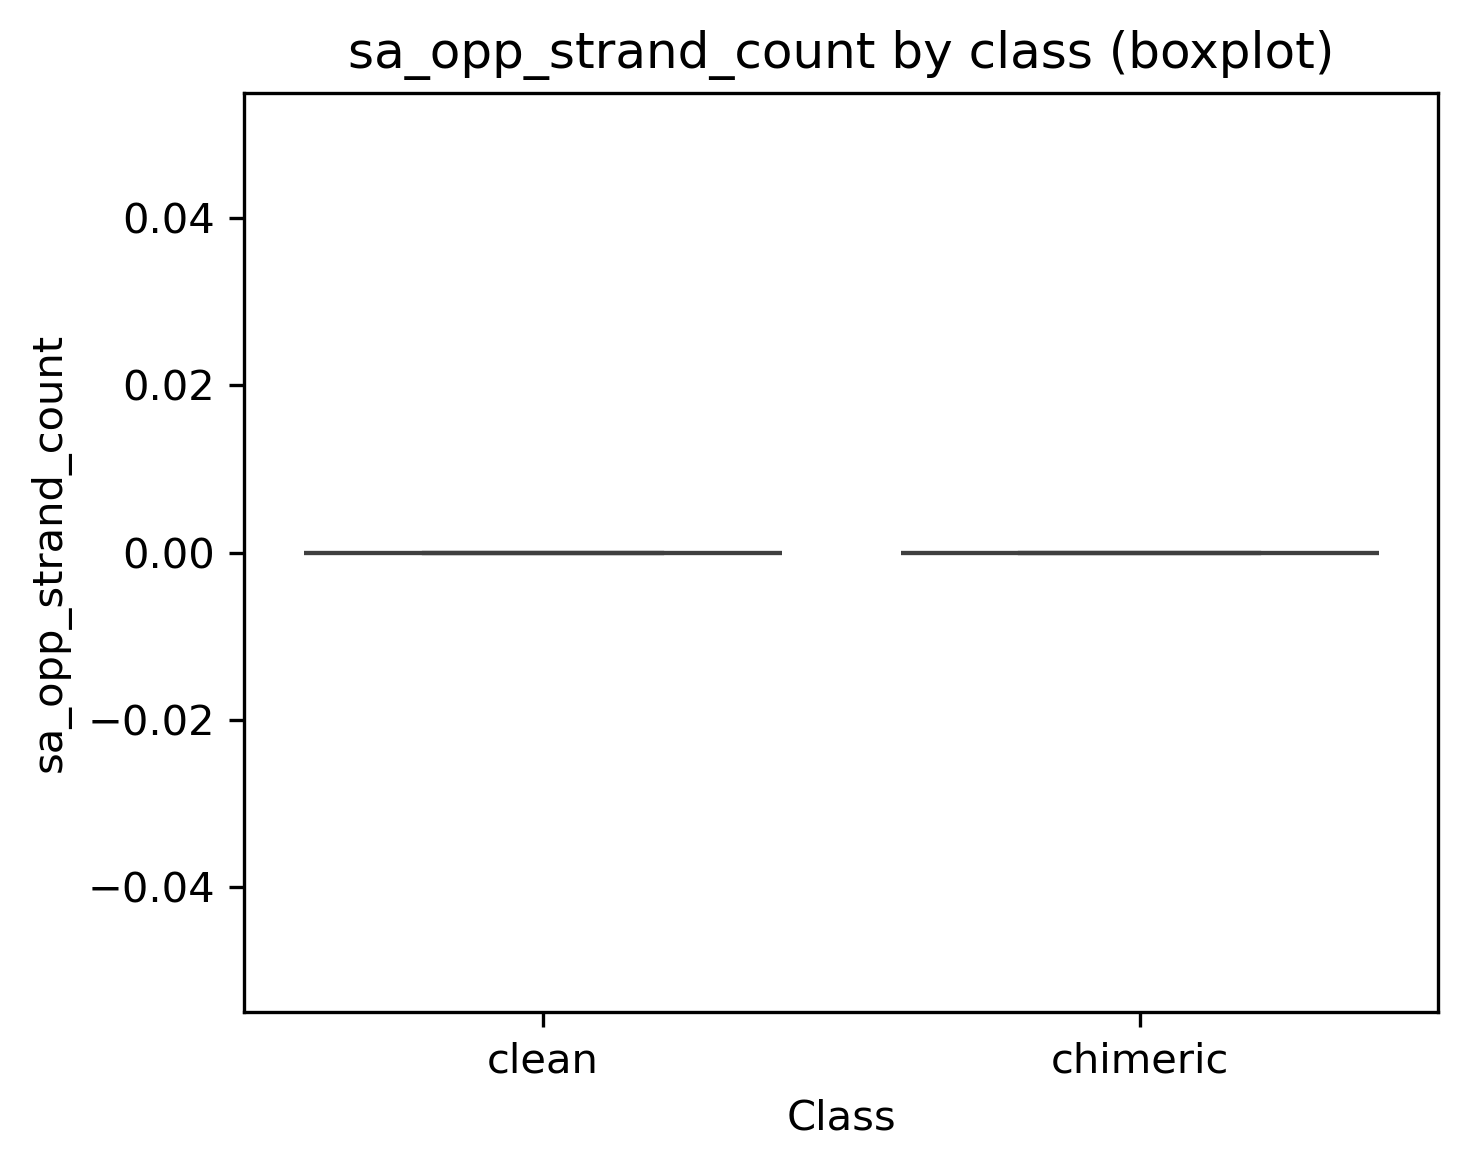
\includegraphics[width=\textwidth]{../notebooks/figures/boxplots/box_sa_opp_strand_count.png}
    \caption{SA opposite strand count}
    \label{fig:app_box_sa_opp_strand_count}
\end{subfigure}

\vspace{0.4em}

\begin{subfigure}[b]{0.32\textwidth}
    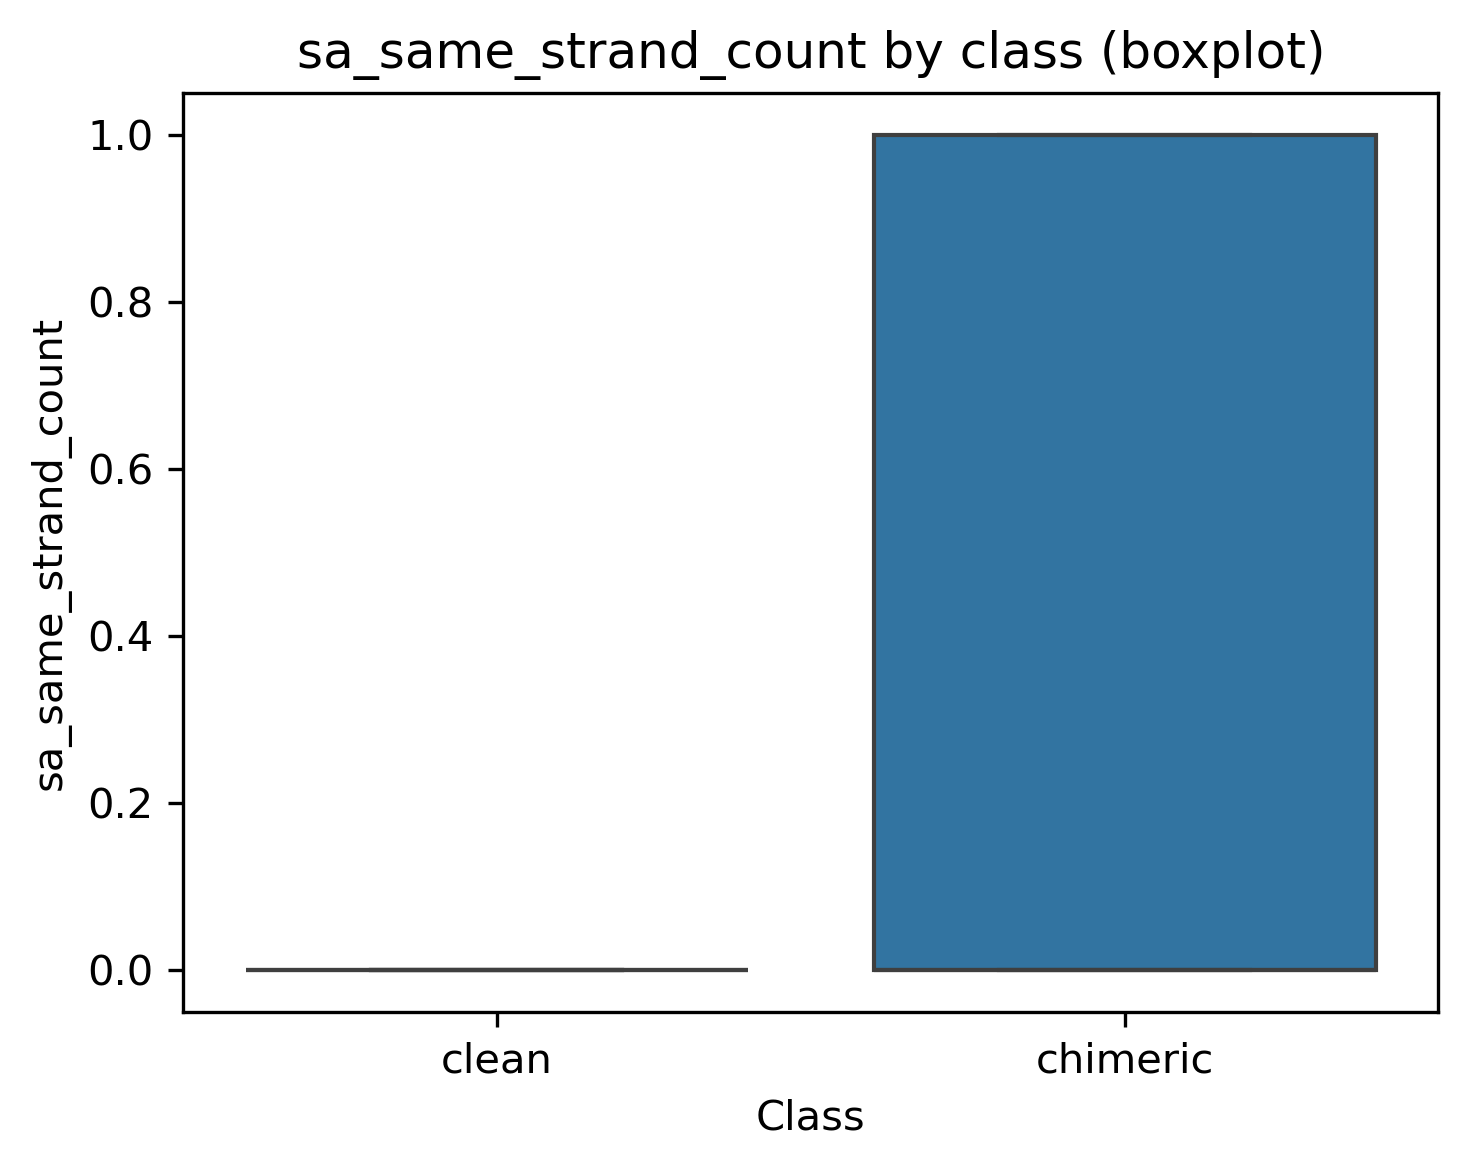
\includegraphics[width=\textwidth]{../notebooks/figures/boxplots/box_sa_same_strand_count.png}
    \caption{SA same strand count}
    \label{fig:app_box_sa_same_strand_count}
\end{subfigure}

\caption{Boxplots of SA Structure features by class (2/2).}
\label{fig:app_sa_structure_boxplots_2}
\end{figure}

\clearpage

\subsection{Clipping-Based Features}
\label{app:boxplots_clipping}

\begin{figure}[!htbp]
\centering
\begin{subfigure}[b]{0.32\textwidth}
    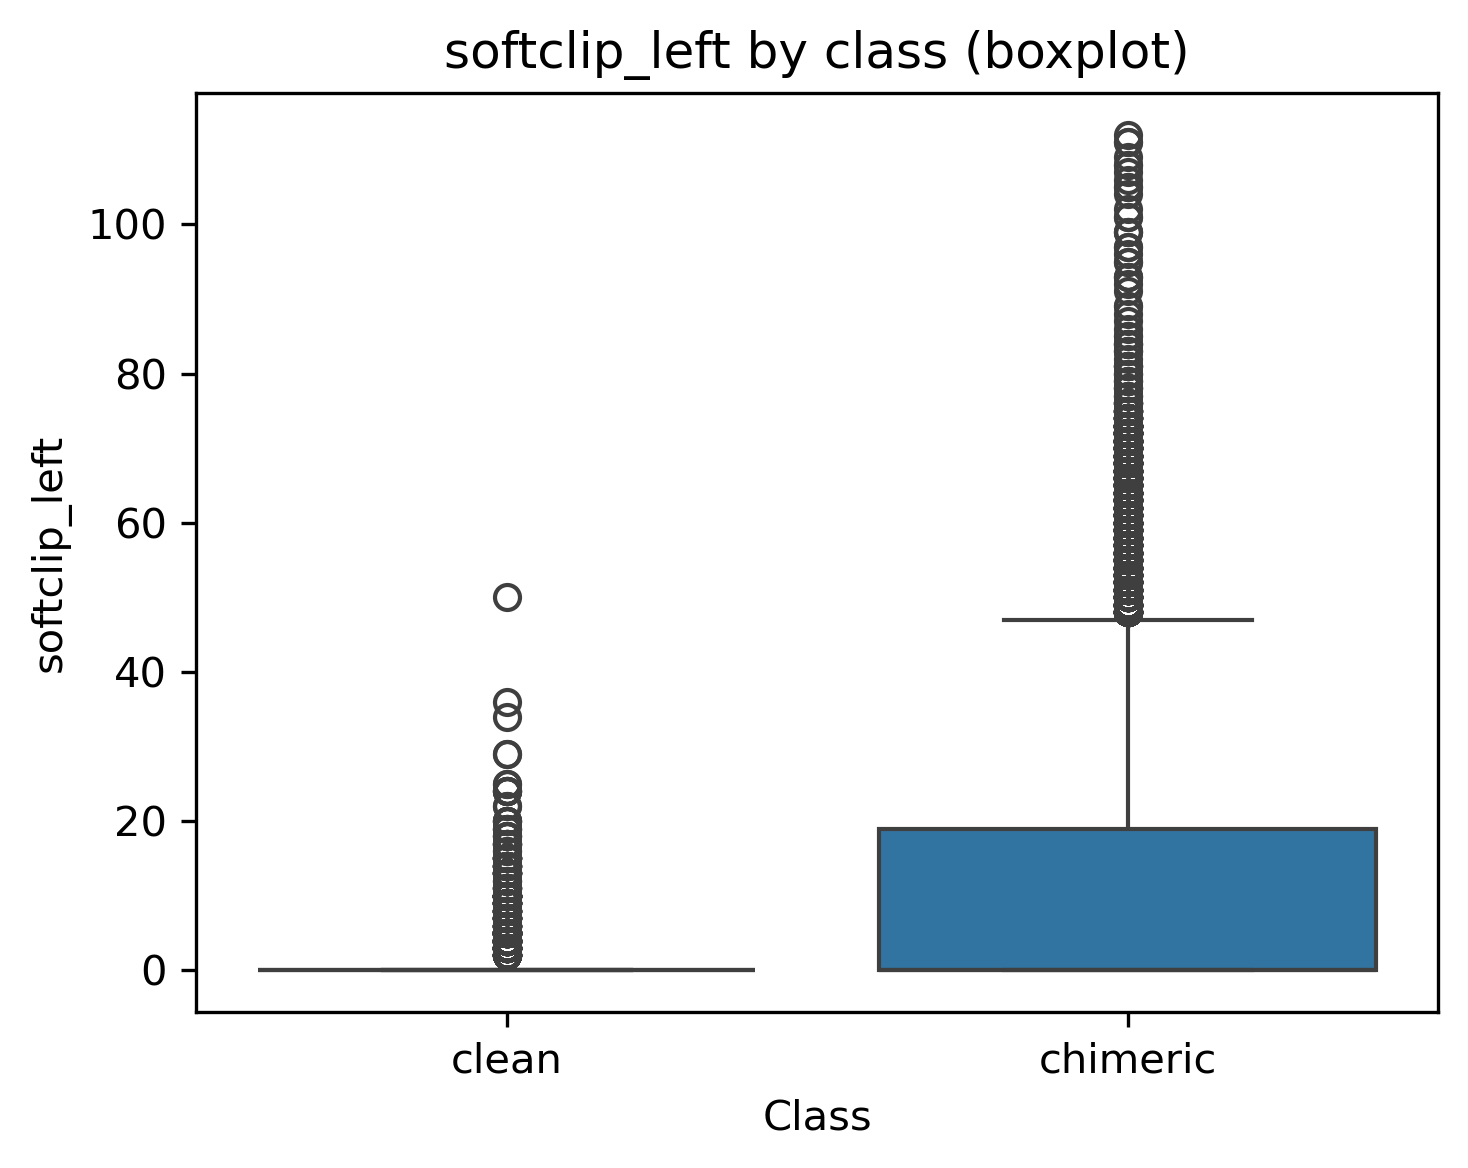
\includegraphics[width=\textwidth]{../notebooks/figures/boxplots/box_softclip_left.png}
    \caption{Softclip left}
    \label{fig:app_box_softclip_left}
\end{subfigure}\hfill
\begin{subfigure}[b]{0.32\textwidth}
    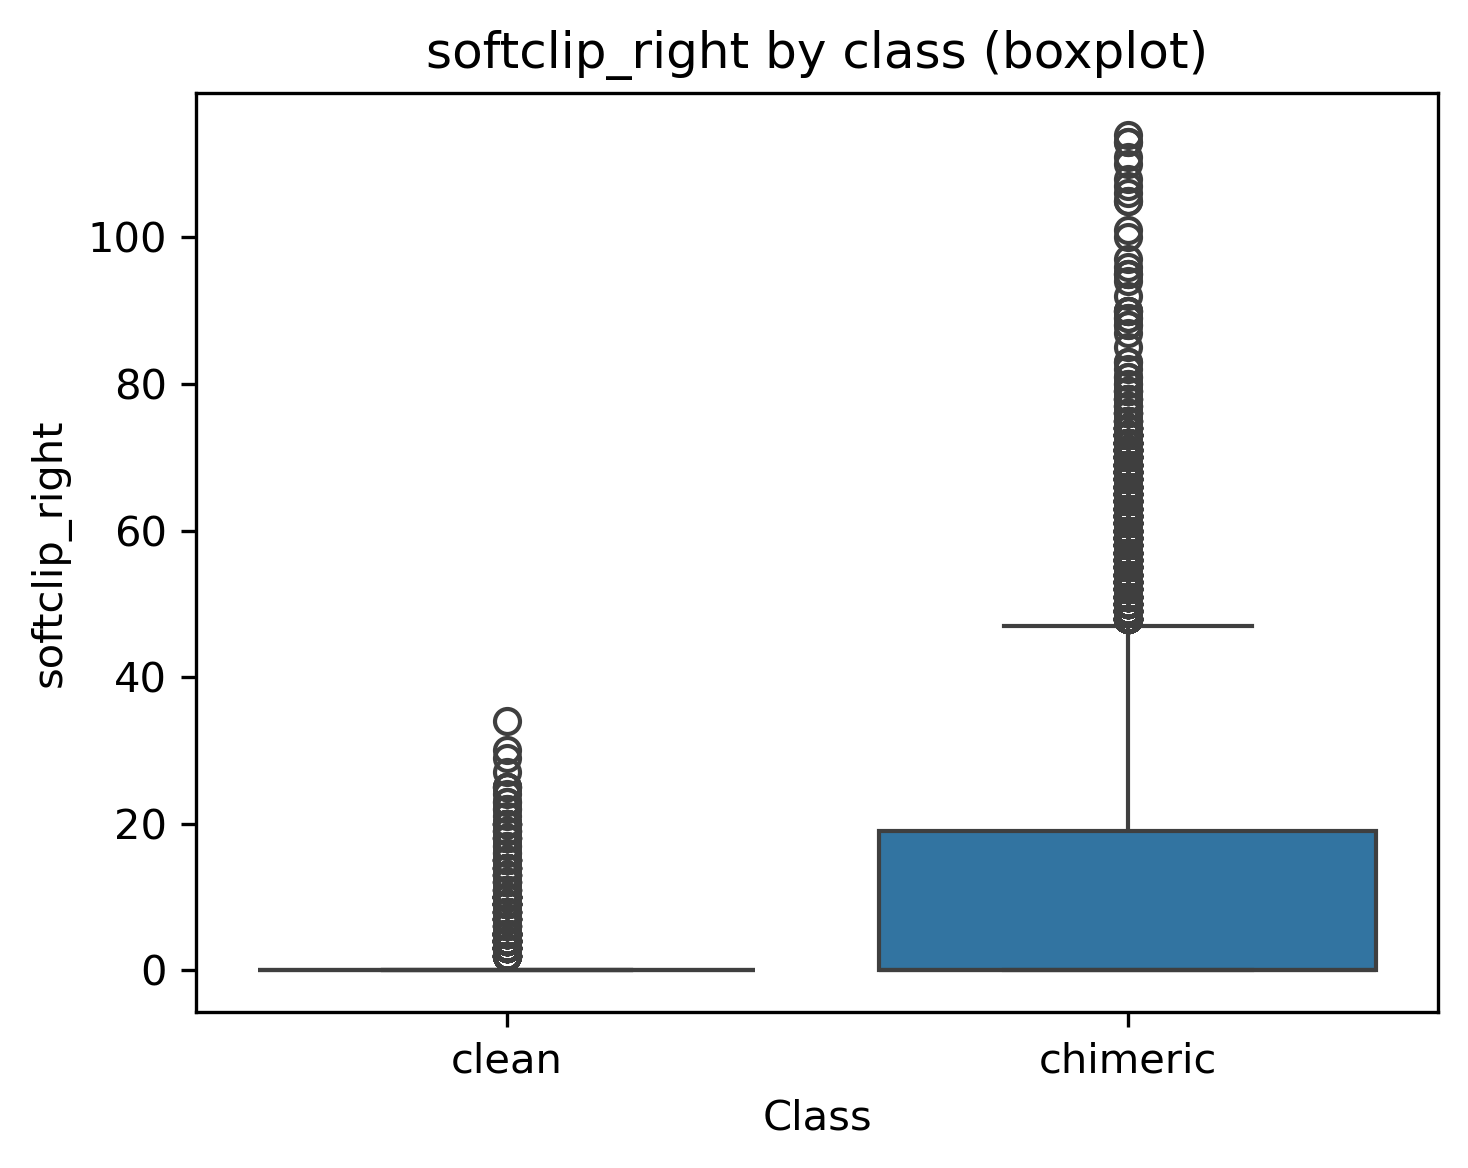
\includegraphics[width=\textwidth]{../notebooks/figures/boxplots/box_softclip_right.png}
    \caption{Softclip right}
    \label{fig:app_box_softclip_right}
\end{subfigure}\hfill
\begin{subfigure}[b]{0.32\textwidth}
    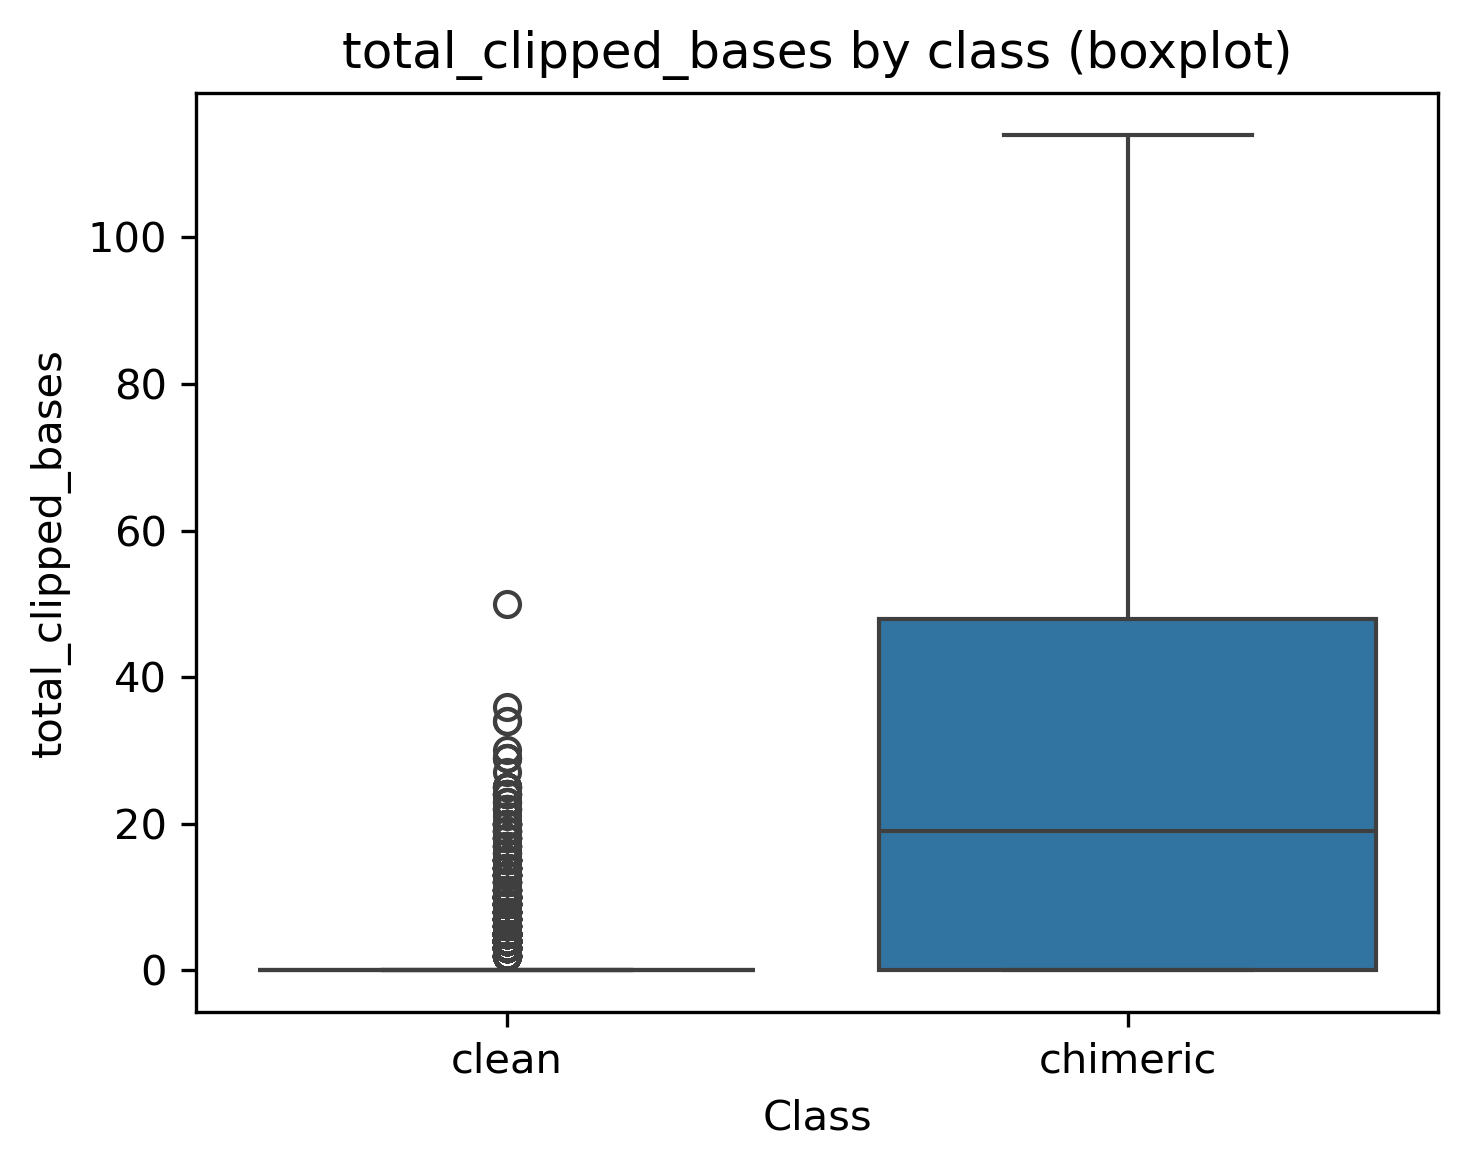
\includegraphics[width=\textwidth]{../notebooks/figures/boxplots/box_total_clipped_bases.png}
    \caption{Total clipped bases}
    \label{fig:app_box_total_clipped_bases}
\end{subfigure}

\caption{Boxplots of clipping-based features by class.}
\label{fig:app_clipping_boxplots}
\end{figure}

\FloatBarrier

\subsection{K-mer Features}
\label{app:boxplots_kmer}

\begin{figure}[!htbp]
\centering
\begin{subfigure}[b]{0.32\textwidth}
    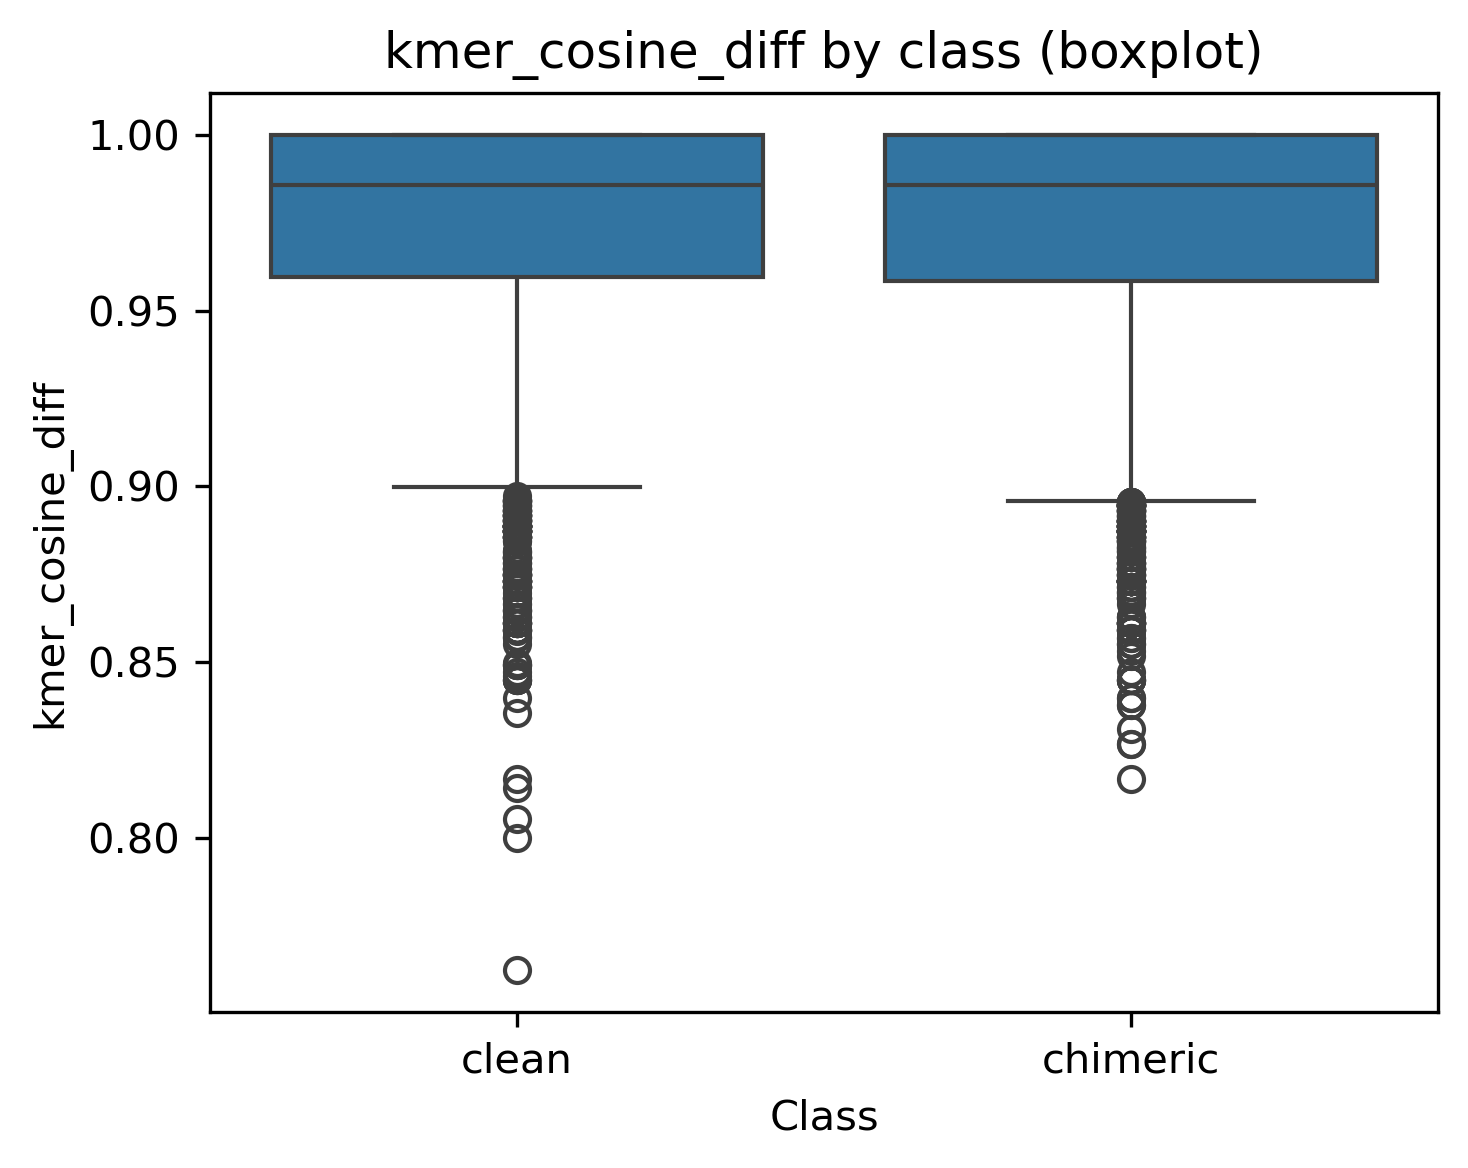
\includegraphics[width=\textwidth]{../notebooks/figures/boxplots/box_kmer_cosine_diff.png}
    \caption{K-mer cosine difference}
    \label{fig:app_box_kmer_cosine_diff}
\end{subfigure}\hfill
\begin{subfigure}[b]{0.32\textwidth}
    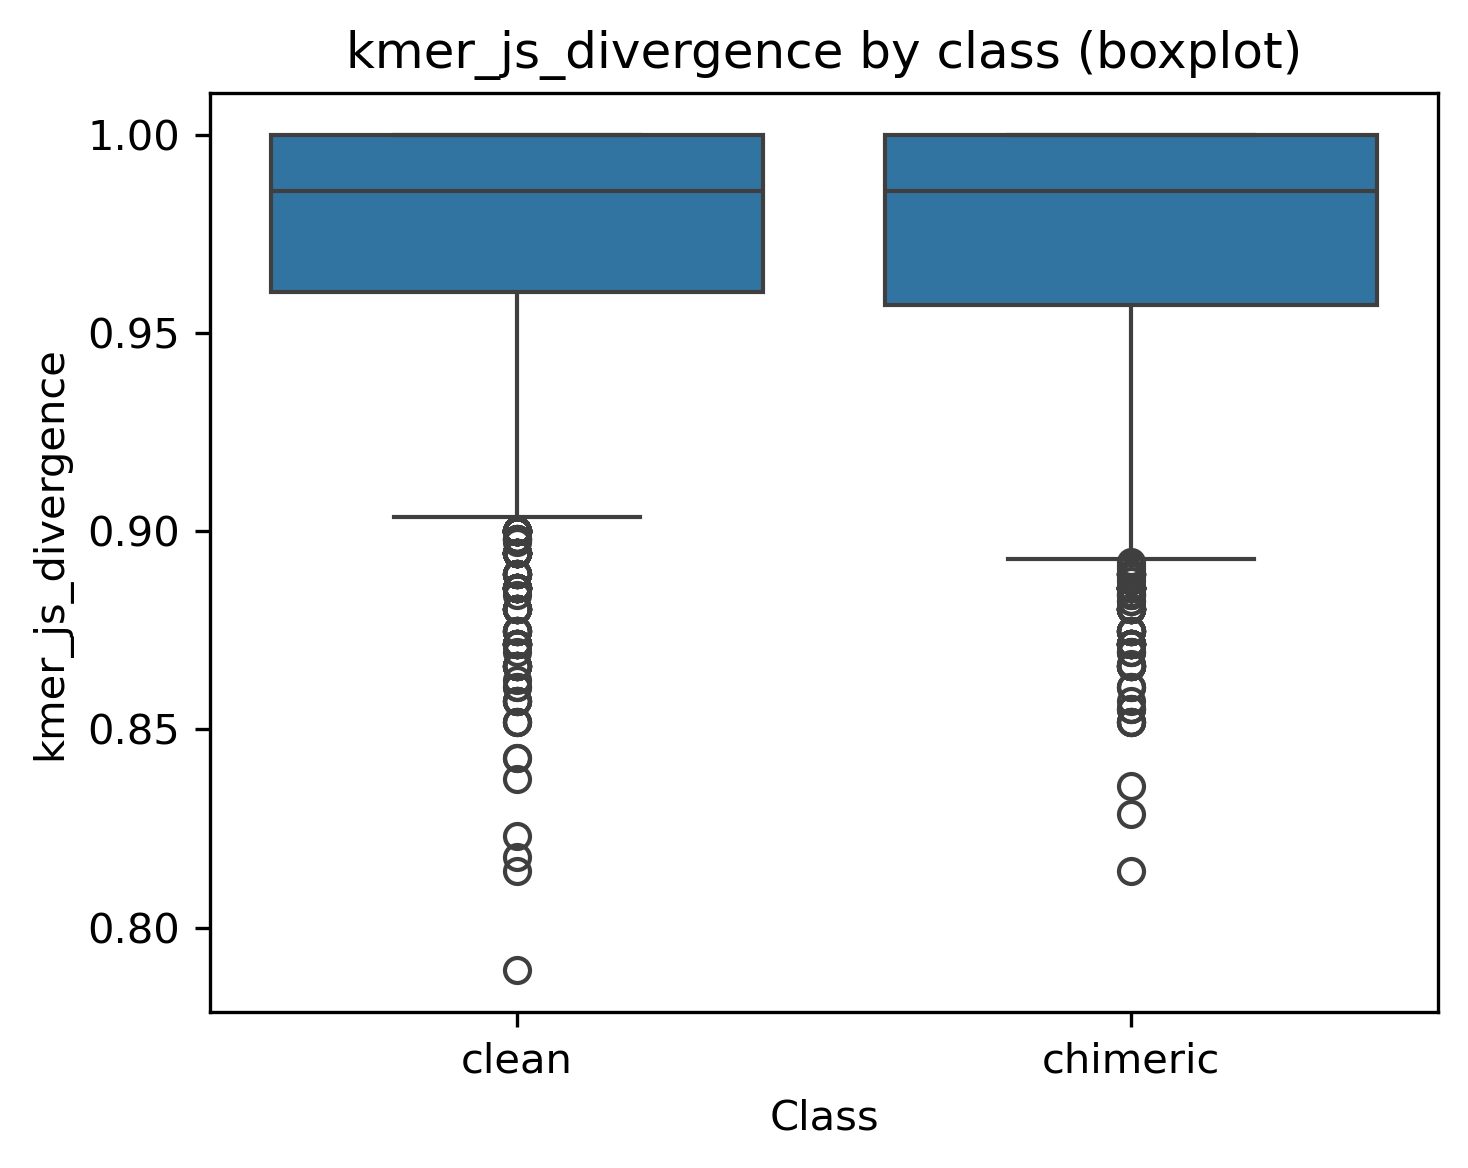
\includegraphics[width=\textwidth]{../notebooks/figures/boxplots/box_kmer_js_divergence.png}
    \caption{K-mer JS divergence}
    \label{fig:app_box_kmer_js_divergence}
\end{subfigure}

\caption{Boxplots of k-mer features by class.}
\label{fig:app_kmer_boxplots}
\end{figure}

\clearpage

\subsection{Microhomology Features}
\label{app:boxplots_microhomology}

\begin{figure}[!htbp]
\centering
\begin{subfigure}[b]{0.32\textwidth}
    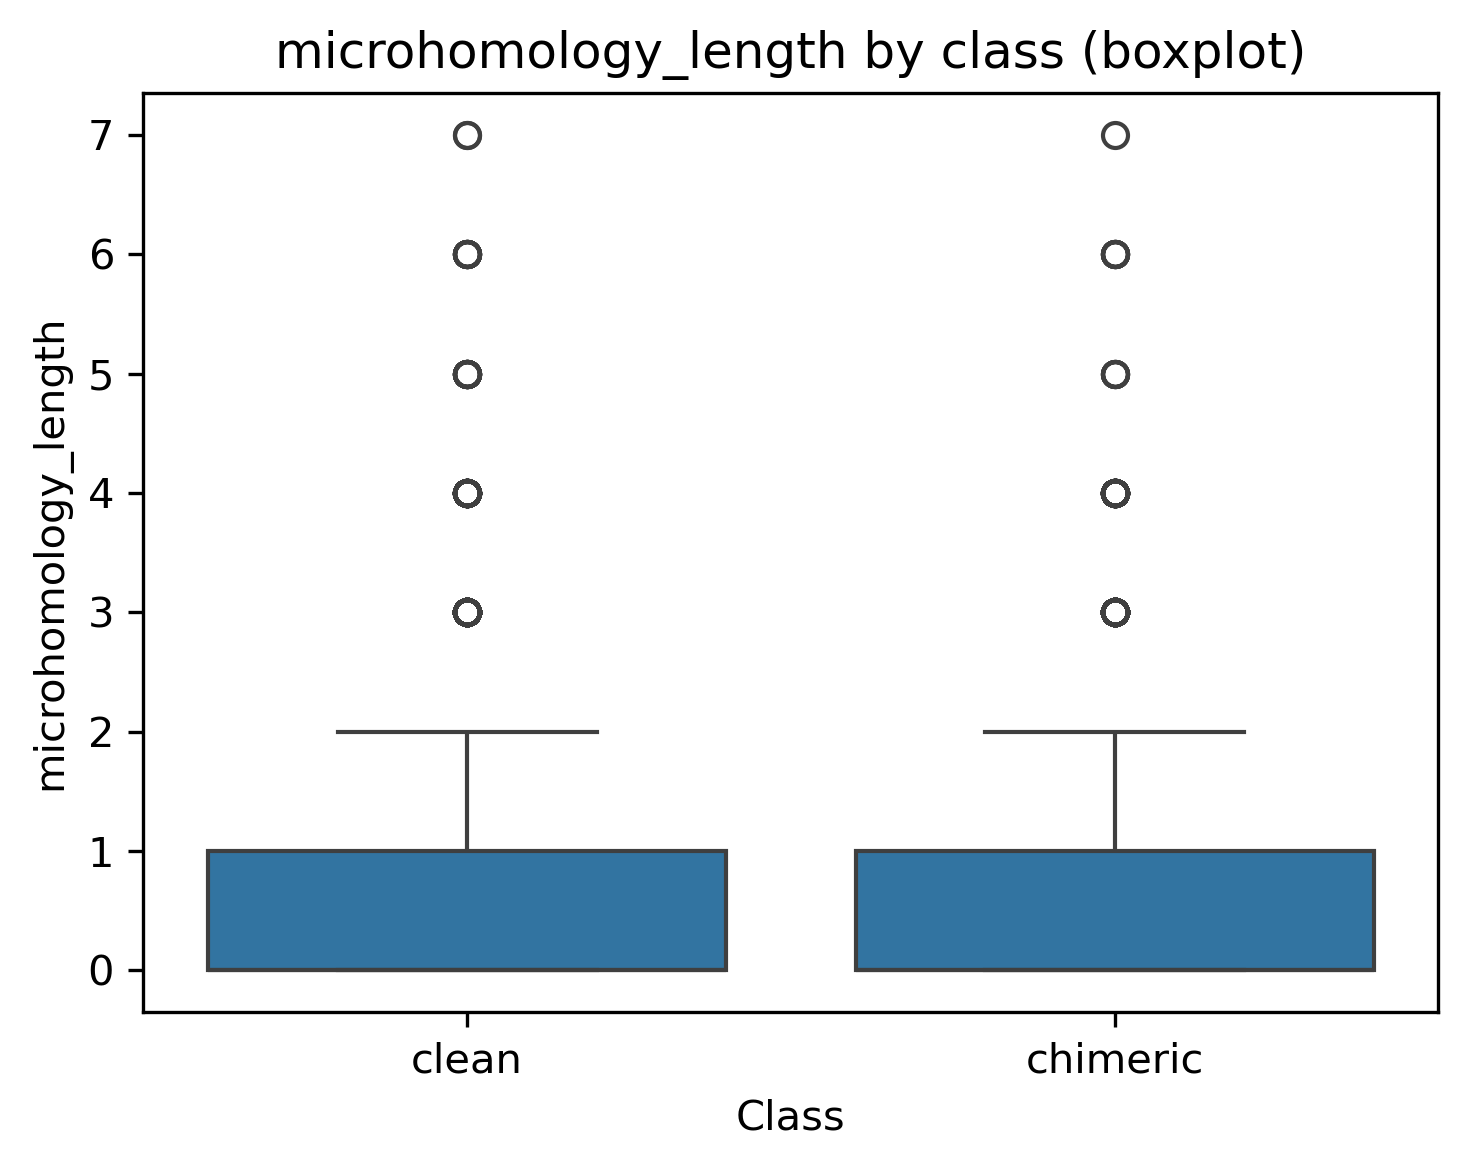
\includegraphics[width=\textwidth]{../notebooks/figures/boxplots/box_microhomology_length.png}
    \caption{Microhomology length}
    \label{fig:app_box_microhomology_length}
\end{subfigure}\hfill
\begin{subfigure}[b]{0.32\textwidth}
    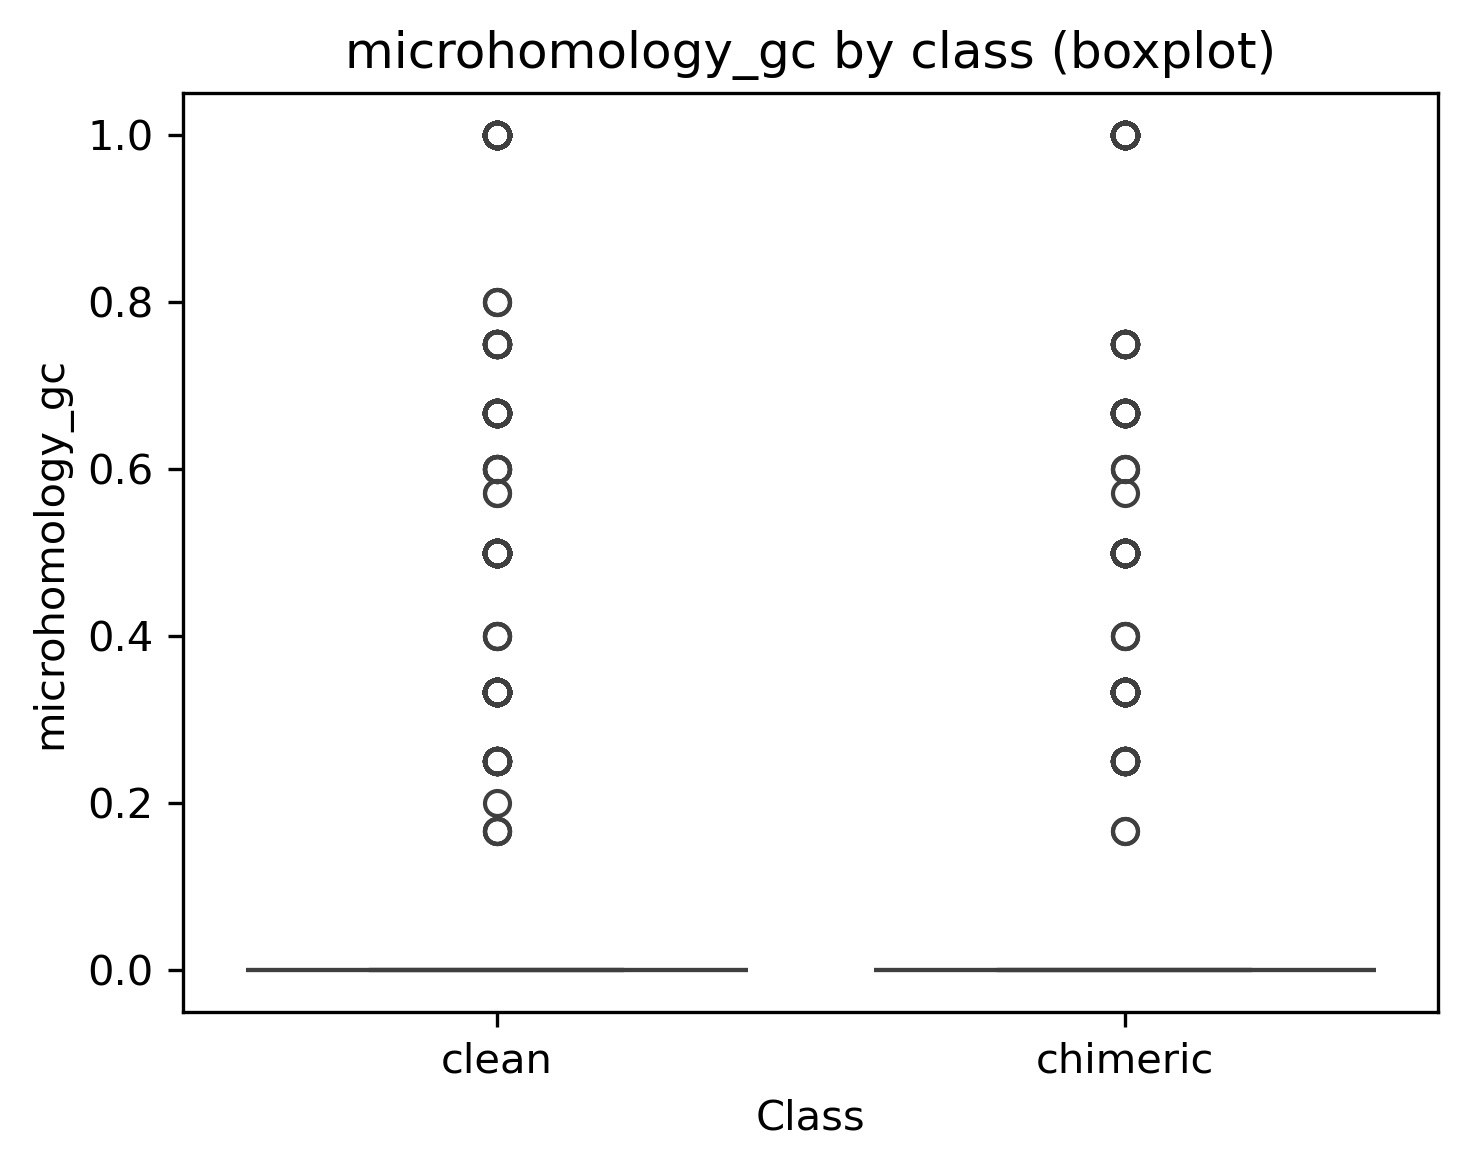
\includegraphics[width=\textwidth]{../notebooks/figures/boxplots/box_microhomology_gc.png}
    \caption{Microhomology GC}
    \label{fig:app_box_microhomology_gc}
\end{subfigure}

\caption{Boxplots of microhomology features by class.}
\label{fig:app_microhomology_boxplots}
\end{figure}

\FloatBarrier

\subsection{Others}
\label{app:boxplots_others}

\begin{figure}[!htbp]
\centering
\begin{subfigure}[b]{0.32\textwidth}
    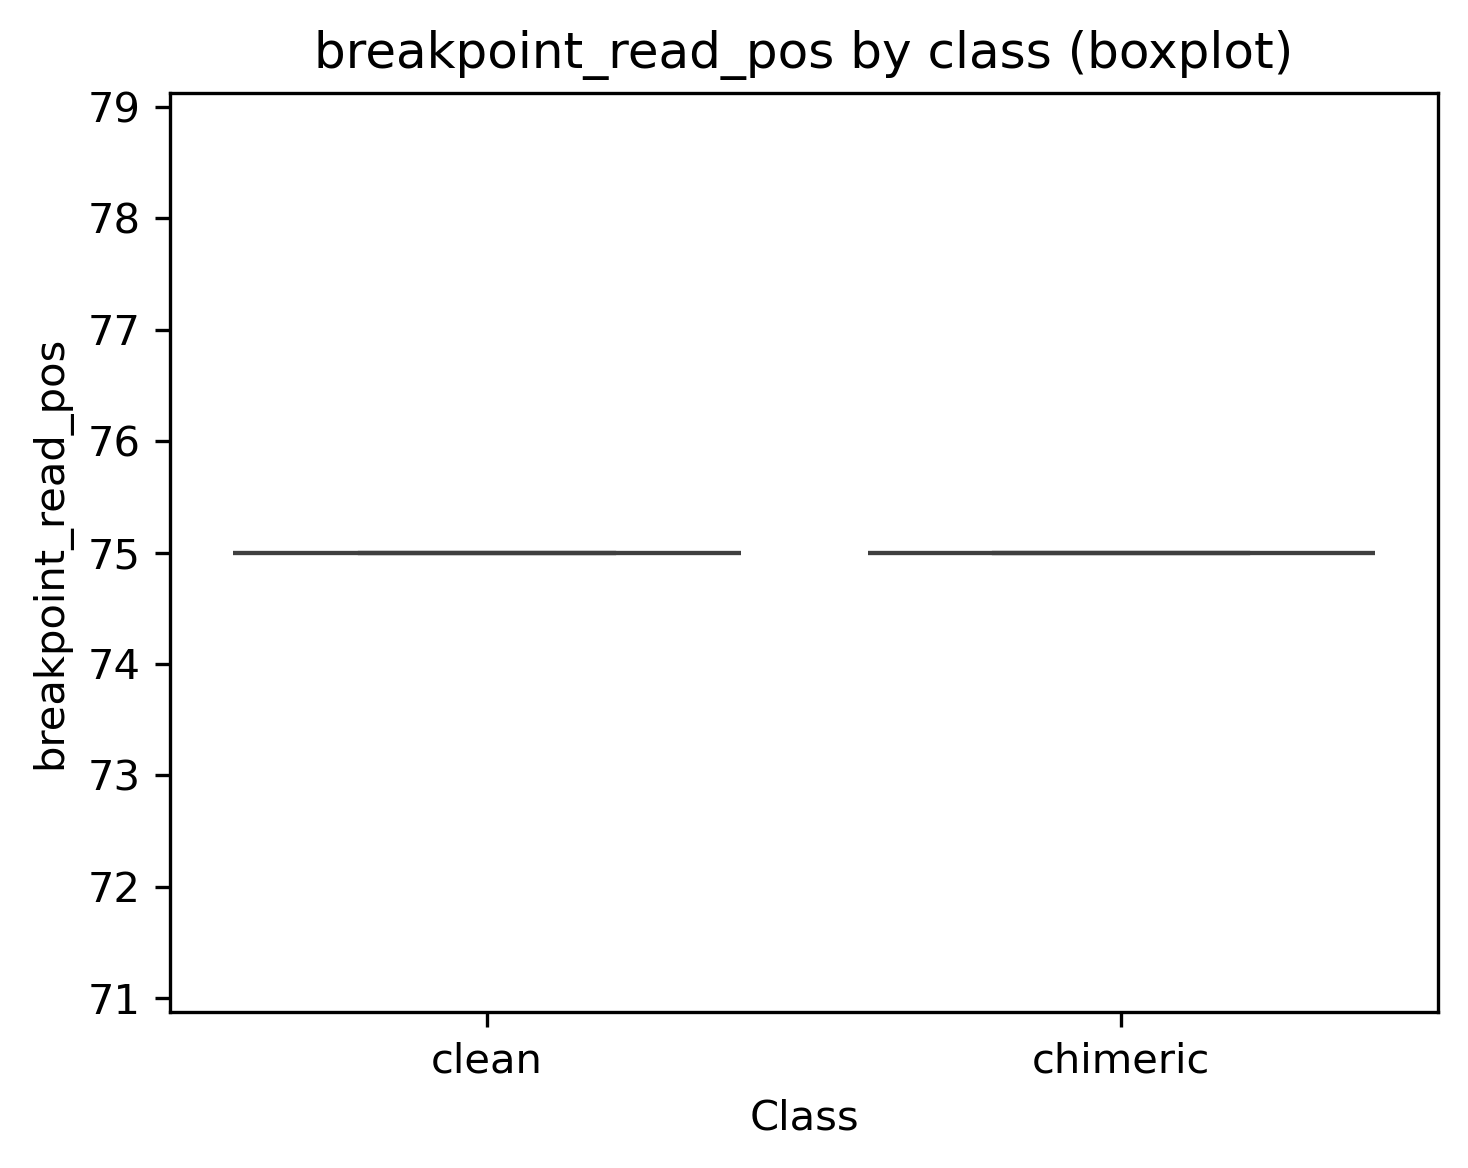
\includegraphics[width=\textwidth]{../notebooks/figures/boxplots/box_breakpoint_read_pos.png}
    \caption{Breakpoint read position}
    \label{fig:app_box_breakpoint_read_pos}
\end{subfigure}\hfill
\begin{subfigure}[b]{0.32\textwidth}
    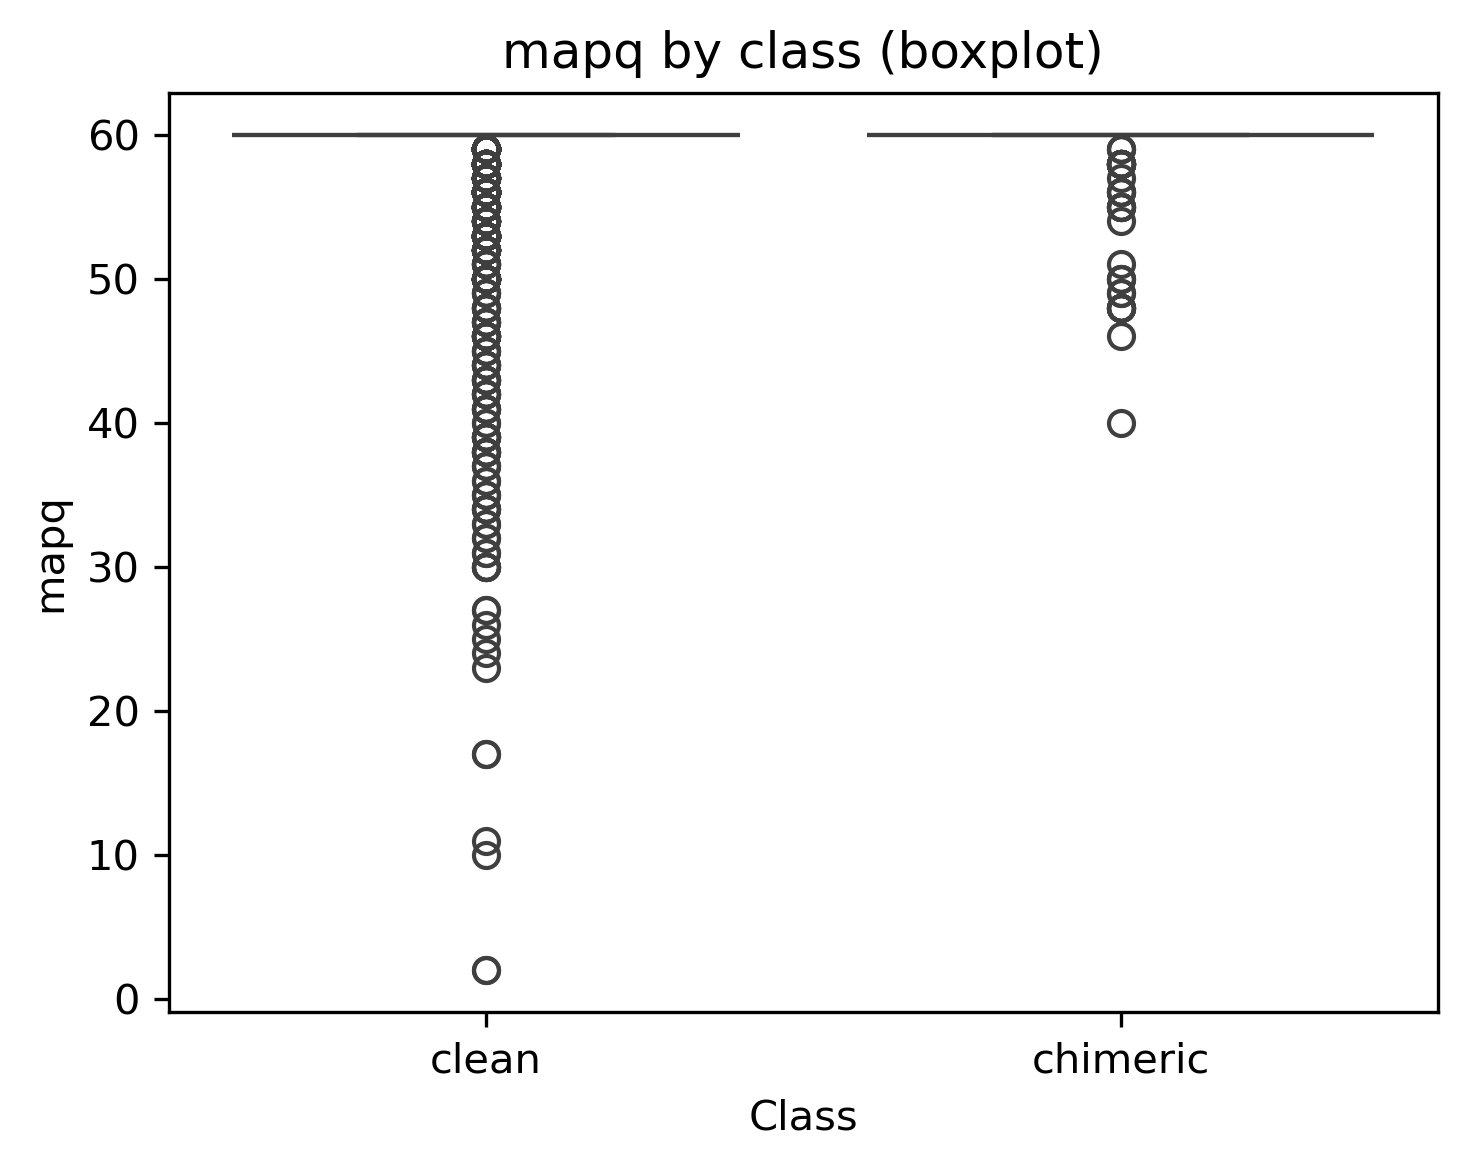
\includegraphics[width=\textwidth]{../notebooks/figures/boxplots/box_mapq.png}
    \caption{MAPQ}
    \label{fig:app_box_mapq}
\end{subfigure}\hfill
\begin{subfigure}[b]{0.32\textwidth}
    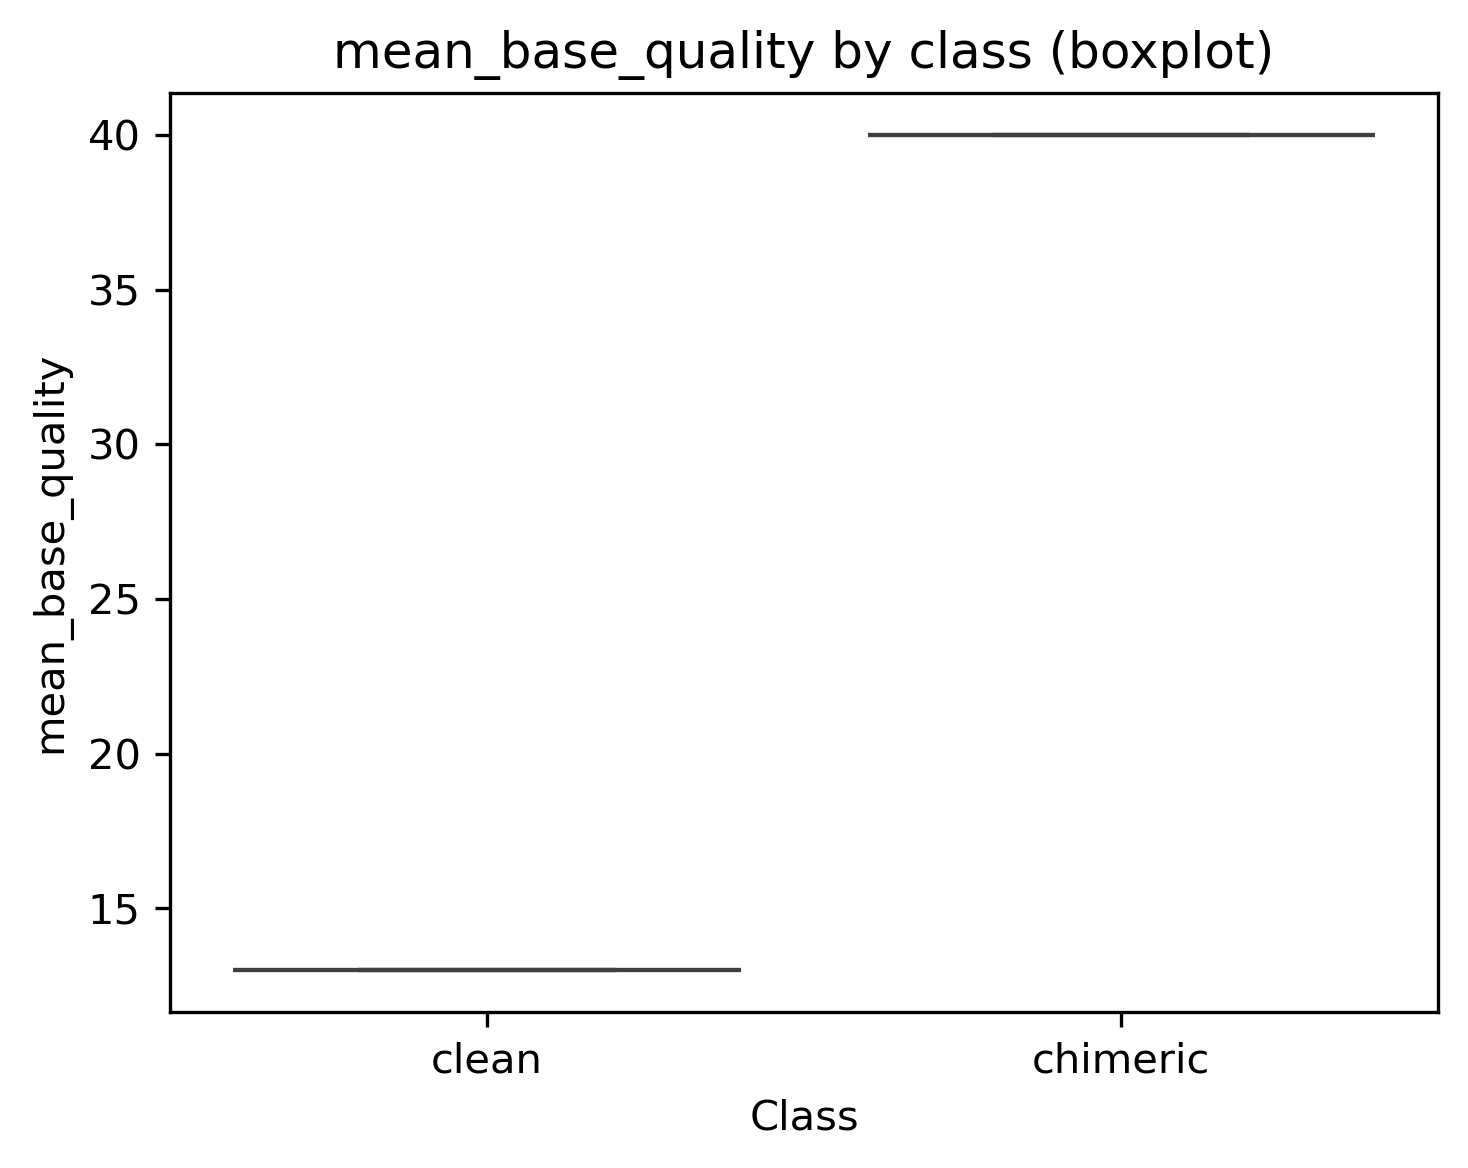
\includegraphics[width=\textwidth]{../notebooks/figures/boxplots/box_mean_base_quality.png}
    \caption{Mean base quality}
    \label{fig:app_box_mean_base_quality}
\end{subfigure}

\vspace{0.4em}

\begin{subfigure}[b]{0.32\textwidth}
    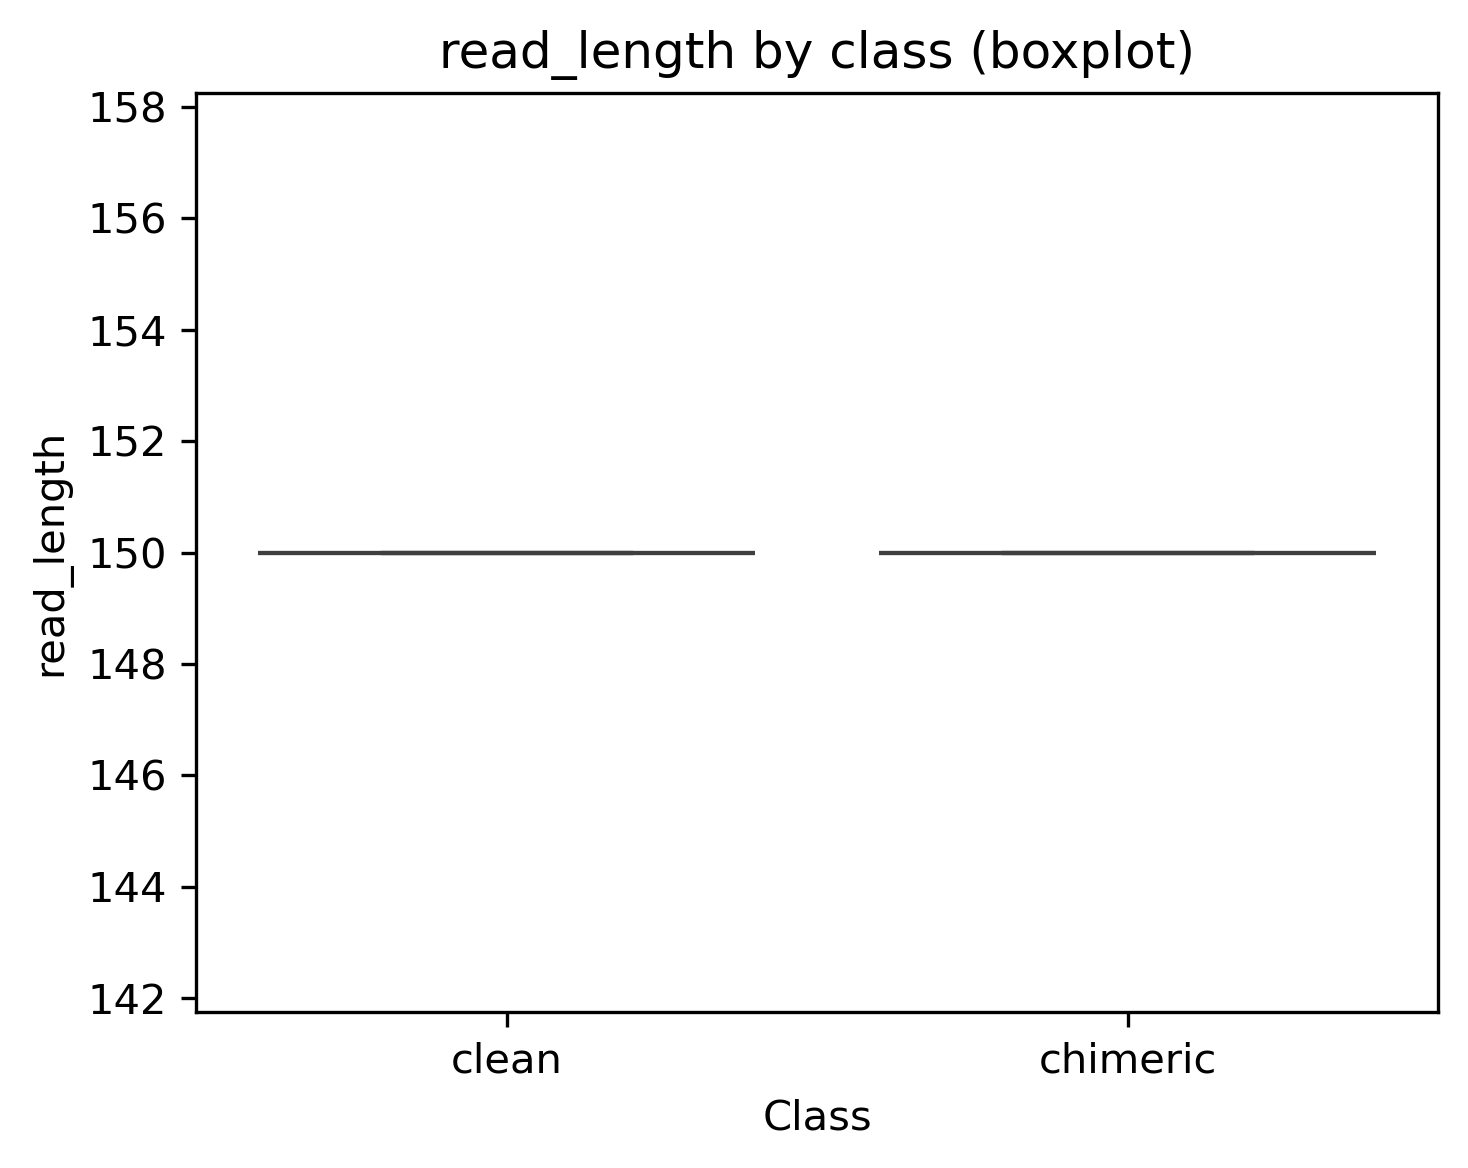
\includegraphics[width=\textwidth]{../notebooks/figures/boxplots/box_read_length.png}
    \caption{Read length}
    \label{fig:app_box_read_length}
\end{subfigure}\hfill
\begin{subfigure}[b]{0.32\textwidth}
    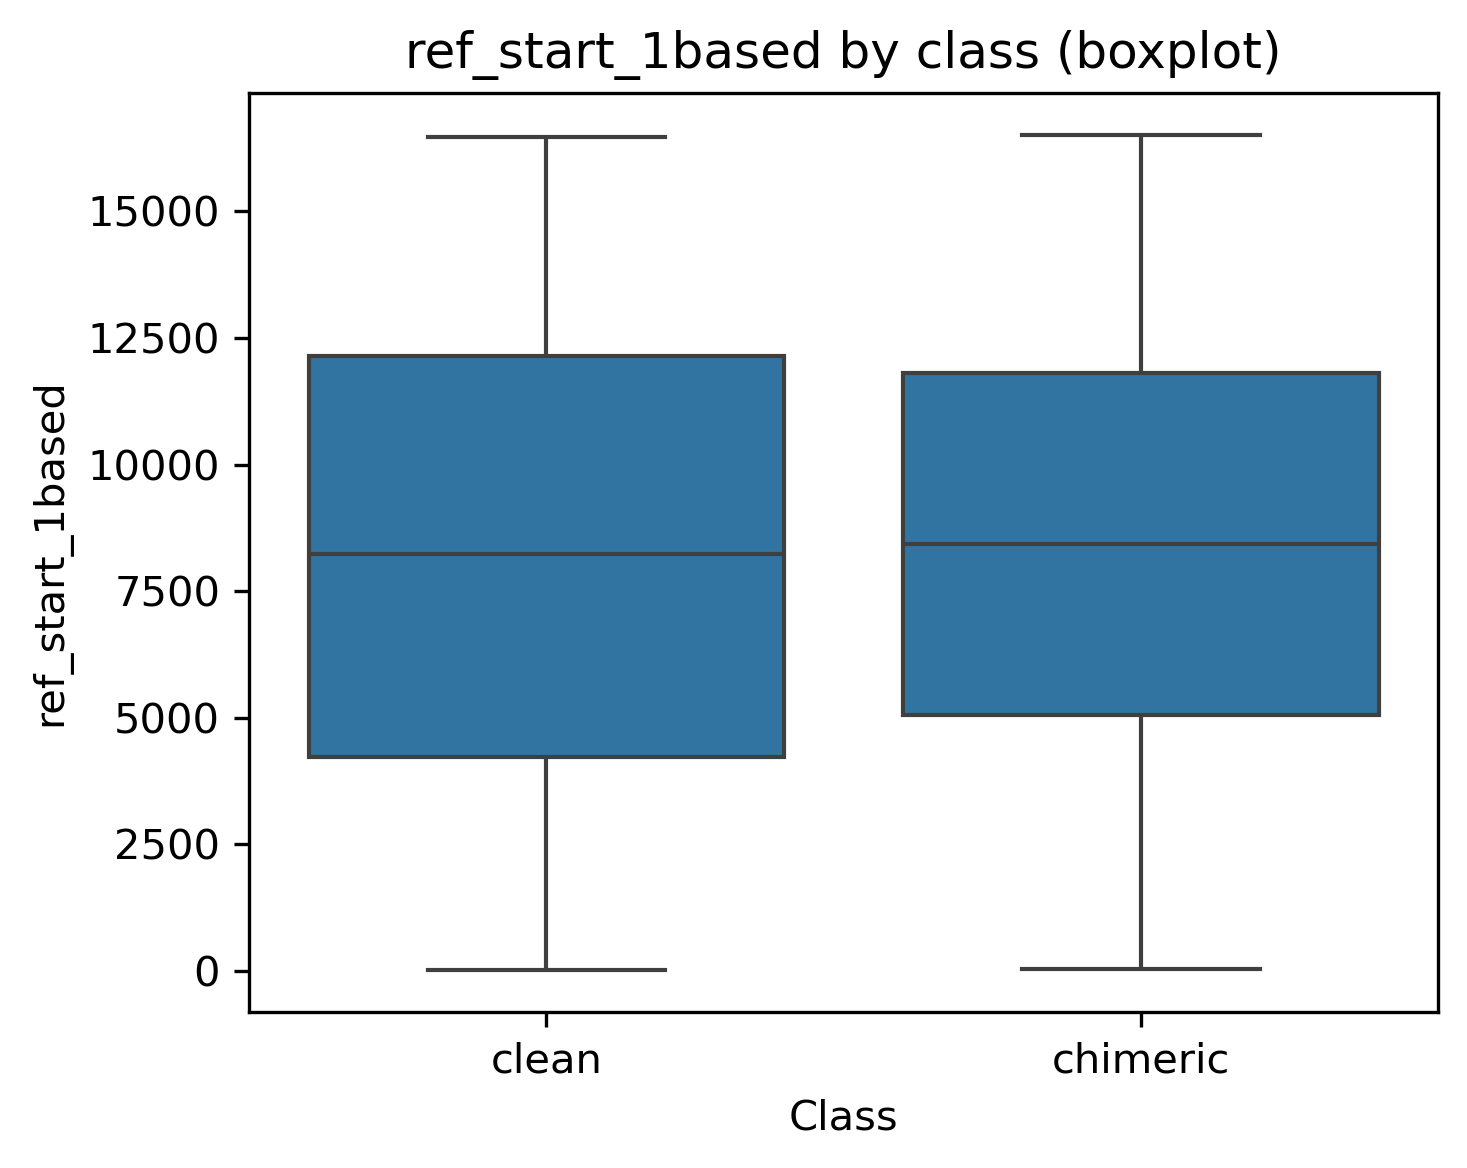
\includegraphics[width=\textwidth]{../notebooks/figures/boxplots/box_ref_start_1based.png}
    \caption{Reference start (1-based)}
    \label{fig:app_box_ref_start_1based}
\end{subfigure}

\caption{Boxplots of other numeric features by class.}
\label{fig:app_others_boxplots}
\end{figure}

\FloatBarrier